\documentclass[12pt,a4paper,twoside,openright]{report}
\usepackage[pdfborder={0 0 0}, breaklinks]{hyperref}    % turns references into hyperlinks
\usepackage[margin=25mm]{geometry}  % adjusts page layout
\usepackage{graphicx}  % allows inclusion of PDF, PNG and JPG images
\usepackage{verbatim}
\usepackage{docmute} 
\usepackage[utf8]{inputenc}
\usepackage[english]{babel}
\usepackage{graphicx}
\usepackage{wrapfig}
\usepackage{float}
\usepackage{booktabs}
\usepackage{tabularx}
\usepackage{multirow}
\usepackage{longtable}
\usepackage{amsmath}
\usepackage{makecell}
\usepackage{amssymb}
\usepackage{calrsfs}
\usepackage{diffcoeff}
\usepackage{mathtools}
\usepackage{amsfonts}
\usepackage{float}
\usepackage[T1]{fontenc}
\usepackage{currvita}
\usepackage[none]{hyphenat}
\usepackage{algorithm}
\usepackage[noend]{algpseudocode}
\usepackage{listings}
\usepackage{xcolor}
\usepackage{natbib}
\usepackage{subcaption}
%\usepackage{breakurl}
\usepackage{url}
\usepackage{fnbreak}

%\usepackage[style=authoryear,backend=biber]{biblatex}
%\addbibresource{refs.bib}

\PassOptionsToPackage{hyphens}{url}

\makeatletter
\def\@documentnocite#1{\@bsphack
	\@for\@citeb:=#1\do{%
		\edef\@citeb{\expandafter\@firstofone\@citeb}%
		\if@filesw\immediate\write\@auxout{\string\citation{\@citeb}}\fi
		\@ifundefined{b@\@citeb}{\G@refundefinedtrue
			\@latex@warning{Citation `\@citeb' undefined}}{}}%
	\@esphack}
\AtBeginDocument{\let\nocite\@documentnocite}

\algdef{SE}[DOWHILE]{Do}{doWhile}{\algorithmicdo}[1]{\algorithmicwhile\ #1}%


\makeatother


\DeclareMathOperator*{\argmax}{arg\,max}
\DeclareMathOperator*{\argmin}{arg\,min}

\setcounter{secnumdepth}{5}
\raggedbottom                           % try to avoid widows and orphans
\sloppy
\clubpenalty1000%
\widowpenalty1000%

\renewcommand{\baselinestretch}{1.1}    % adjust line spacing to make
                                        % more readable
      
      
 \colorlet{punct}{red!60!black}
 \definecolor{background}{HTML}{EEEEEE}
 \definecolor{delim}{RGB}{20,105,176}
 \colorlet{numb}{magenta!60!black}
                                   
 \lstdefinelanguage{json}{
 	basicstyle=\normalfont\ttfamily,
 	numbers=left,
 	numberstyle=\scriptsize,
 	stepnumber=1,
 	numbersep=8pt,
 	showstringspaces=false,
 	breaklines=true,
 	frame=lines,
 	backgroundcolor=\color{white},
 	literate=
 	*{0}{{{\color{numb}0}}}{1}
 	{1}{{{\color{numb}1}}}{1}
 	{2}{{{\color{numb}2}}}{1}
 	{3}{{{\color{numb}3}}}{1}
 	{4}{{{\color{numb}4}}}{1}
 	{5}{{{\color{numb}5}}}{1}
 	{6}{{{\color{numb}6}}}{1}
 	{7}{{{\color{numb}7}}}{1}
 	{8}{{{\color{numb}8}}}{1}
 	{9}{{{\color{numb}9}}}{1}
 	{:}{{{\color{punct}{:}}}}{1}
 	{,}{{{\color{punct}{,}}}}{1}
 	{\{}{{{\color{delim}{\{}}}}{1}
 	{\}}{{{\color{delim}{\}}}}}{1}
 	{[}{{{\color{delim}{[}}}}{1}
 	{]}{{{\color{delim}{]}}}}{1},
 }

%\g@addto@macro{\UrlBreaks}{\UrlOrds}
 
 \interfootnotelinepenalty=0
\begin{document}


\bibliographystyle{plain}


%%%%%%%%%%%%%%%%%%%%%%%%%%%%%%%%%%%%
%%%%%%%%%%%%%%% TITLE %%%%%%%%%%%%%%%%%
%%%%%%%%%%%%%%%%%%%%%%%%%%%%%%%%%%%%

\pagestyle{empty}

\rightline{\LARGE \textbf{Tudor Mihai Avram}}

\vspace*{60mm}
\begin{center}
	\Huge
	\textbf{Machine learning graph filtering} \\[5mm]
	Computer Science Tripos -- Part II \\[5mm]
	Homerton College \\[5mm]
	\today  % today's date
\end{center}

%%%%%%%%%%%%%%%%%%%%%%%%%%%%%%%%%%%%
%%%%%%%%%%%% PROFORMA %%%%%%%%%%%%%%%%
%%%%%%%%%%%%%%%%%%%%%%%%%%%%%%%%%%%%

\pagestyle{plain}

\chapter*{Proforma}

{\large
	\begin{tabular}{ll}
		Name:               & \bf Tudor Mihai Avram                     \\
		College:            & \bf Homerton College                    \\
		Project Title:      & \bf Machine learning graph filtering \\
		Examination:        & \bf Computer Science Tripos -- Part II, July 2018  \\
		Word Count:         & \bf 1\footnotemark[1] \\
		Project Originator: & Dr Ripduman Sohan                   \\
		Supervisor:         & Dr Lucian Carata                    \\ 
	\end{tabular}
}

\footnotetext[1]{This word count was computed
	by \texttt{detex dissertation.tex | tr -cd '0-9A-Za-z $\tt\backslash$n' | wc -w}
}

\section*{Original aims of the project}
\section*{Work completed}
\section*{Special Difficulties}

\newpage

\section*{Declaration}

%%%%%%%%%%%%%%%%%%%%%%%%%%%%%%%%%%%%
%%%%%%%% TABLE OF CONTENTS %%%%%%%%%%%%%
%%%%%%%%%%%%%%%%%%%%%%%%%%%%%%%%%%%%

\tableofcontents

%%%%%%%%%%%%%%%%%%%%%%%%%%%%%%%%%%%%
%%%%%%%%%%%% LIST OF FIGURES %%%%%%%%%%%%%
%%%%%%%%%%%%%%%%%%%%%%%%%%%%%%%%%%%%

\listoffigures

%%%%%%%%%%%%%%%%%%%%%%%%%%%%%%%%%%%%
%%%%%%%%%%%% LIST OF TABLES %%%%%%%%%%%%%
%%%%%%%%%%%%%%%%%%%%%%%%%%%%%%%%%%%%

\listoftables

%%%%%%%%%%%%%%%%%%%%%%%%%%%%%%%%%%%%
%%%%%%%%%%%%  INTRODUCTION %%%%%%%%%%%%%
%%%%%%%%%%%%%%%%%%%%%%%%%%%%%%%%%%%%

\begin{document}
	
	\chapter{Introduction}
	
	This dissertation explores how machine learning techniques can be applied for determining important nodes (according to set criteria) in large graphs, allowing their interactive exploration. This problem is particularly important for provenance graphs describing abstractions at the operating system level. A provenance graph accurately records the history of all interactions between objects such as files, processes, sockets and pipes on a given machine. When using such graphs for identifying potential attacks(network intrusion, sensitive data exfiltration) on systems, an analyst would need to sift through large and potentially irrelevant parts of the graph in search for suspicious activity. This project aims to provide a tool for helping the analyst in this task. To that end, I implemented and comparatively evaluated a number of machine learning models that classify nodes as being of interest or not. On top of these classifiers, I also implemented a server infrastructure that facilitates communication between the model and the client (see section \ref{1.2}). This allows the UI clients to access the predictions of the model with respect to node relevancy. 
	
	\section{Aims \& Motivation}  \label{1.1}
	Analysing event logs of a distributed system to identify actionable security information and hence to act accordingly in order to improve a system's security has always been a desirable goal for both research and industry. The availability of cheap data storage facilitated such large scale logs collection, on the order of several terabytes of data, making manual log reviewing an unfeasible task. 
	\\ \\
	Moreover, computer logs are becoming more structured. Using graphs to highlight the relationships between various records inside logs introduces a whole new dimension in terms of richness of the information that needs to be explored. Automatically processing such graphs in order to extract useful information can be difficult, as graphs cannot be directly provided as input to machine learning algorithms.
	
	\subsection{Overview of CADETS UI}\label{1.1.1}
	This project is an extension of the CADETS user interface, a cybersecurity provenance analysis tool developed as part of the CADETS and OPUS research projects. It displays OS-level abstractions as a network, emphasising the relationships between actors(processes, users) and objects(files, sockets, pipes). It is the analyst's task to explore this network in order to identify potentially suspicious nodes(i.e. nodes describing activities done by an attacker). 
	\\ \\
	In order to provide comprehensive data from which the analyst can infer useful information, the network will have a large number of nodes. This makes exploring the entire dataset very difficult for humans.  For example, tracing done on two machines for 7 minutes can produce as many as 6,000 nodes in the network. As the number of machines and the time interval we do tracing on increase, this number will become considerably larger, presenting a significant scalability issue when it comes to manual reviewing. Therefore, it is imperative to filter these nodes in order to give the analyst any hope of finding relevant patterns.
	\begin{figure}[H]
		\centering
		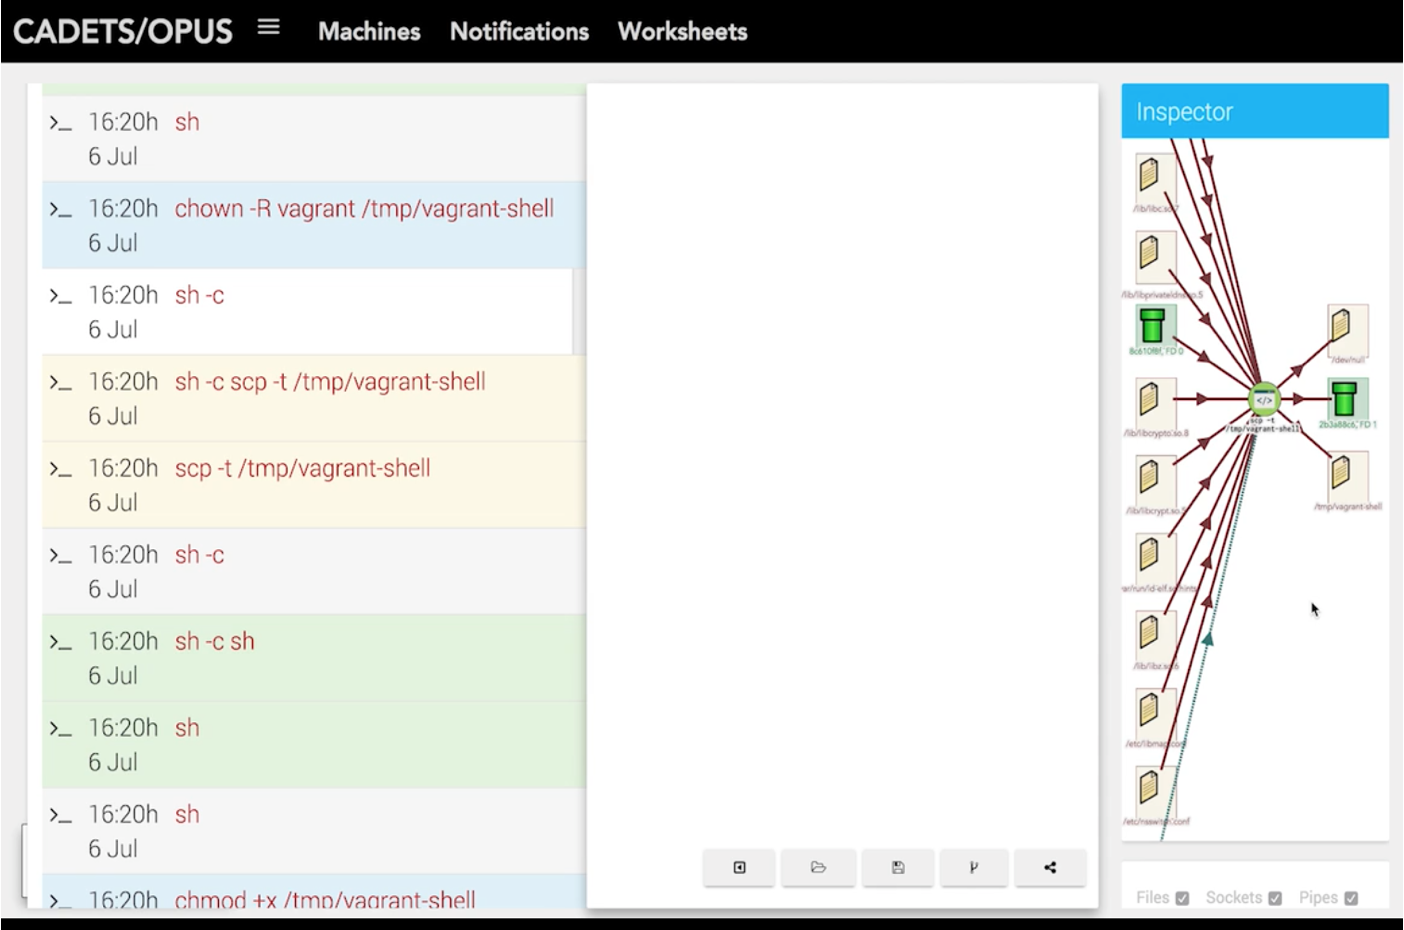
\includegraphics[width=0.7\textwidth]{graphics/CADETS}
		\caption{Snapshot of CADETS UI}
		\label{Figure 1.1}
	\end{figure}
	
	\subsection{Aims of the project}
	In general, the number of nodes that are of interest is lower than the number of nodes that are not. Therefore, the aim of this project is to asses the suitability of different machine learning algorithms that would significantly improve the analyst's experience by reducing the number of nodes he would have to manually inspect. 
	
	\section{Overview of the architecture}\label{1.2}
	The project's main component is a supervised learning algorithm that classifies nodes from the graph as being of interest or not. The model is optimised using a labelled training set constructed based on a set of predefined ground-truths.
	\\ \\
	The communications between the CADETS UI and the machine learning model is facilitated by a REST API(as shown in Figure \ref{Figure 1.2}). For performance purposes, it caches previous classifications locally. 
	\\ \\ 
	When it receives a request from the client, the server would first check the local cache. If it can find the classification result for that node, then it just returns the cached value to the client.
	\begin{figure}[H]
		\centering
		\includegraphics[width=0.8\textwidth]{graphics/overview}
		\caption{Overview of the project's architecture}
		\label{Figure 1.2}
	\end{figure}
	
	If the result is not in the cache or if the cached value is out of date, it runs the machine learning model in order to classify that specific node. Once the classification is done, the result is stored in the local cache and returned to the client. 
	
	\section{Related work}
	Cybersecurity has always been a major concern in computer science, both in industry and in research. With the recent interest shown in artificial intelligence and machine learning, there have been an increasing number of tools that use related methodologies to identify malicious behaviour. The first 
	part of this section will describe a general purpose intrusion detection system, while the following two outline tools that use machine learning in order to identify potentially malicious behaviour.
	
	\subsection{Intrusion detection systems}
	An intrusion detection system(IDS) is a system that monitors traffic for suspicious activity and issues alerts when such activity is discovered. While anomaly detection and reporting is their primary functionality, some IDSs are also capable of taking action when malicious activity or anomalous traffic is detected. 
	\\ \\
	There are numerous IDSs currently available. Snort\footnote{\textbf{\url{https://www.snort.org/}}} is one of the leading such tools with continued development both from the open source community and its corporate parent, Sourcefire Inc. It can detect probes or attacks, such as operating system fingerprinting (i.e. an attacker identifying the OS that runs on a specific machine). 
	\\ \\
	Although they work reasonably well for personal use, traditional IDSs fail to stem the tide of attacks aiming at encrypting or destructing critical data when it comes to large scale systems. Therefore, a pressing need for new monitoring and analysis tools that reduce both false-positive rates and the cognitive burden on human analysts arises. The CADETS UI is such a system and, using the extension implemented as part of this project, it will considerably reduce the amount of manual analysis required. 
	
	\subsection{Clearcut}
	Clearcut\footnote{\textbf{\url{https://github.com/DavidJBianco/Clearcut}}} is an open source tool that uses machine learning techniques for incident detection. It takes HTTP proxy logs as input and filters them, in order to aid the analyst in manually reviewing them. 
	\\ \\ 
	The algorithm used in this case is Random Forest Classification, which uses multiple decision trees. The resulting class corresponding to the mode of the classes returned by the decision trees running separately. 
	\\ \\
	Compared to Clearcut, the inputs for the project described in this dissertation have a graph structure, taking into consideration the logs as well as the relationships between them. This adds a new level of complexity to the problem I am trying to solve.
	
	\subsection{Polonium}
	Polonium is a scalable and effective technology that uses graph mining for malware detection. The tool uses a bipartite graph whose nodes describe machines and files as its training data. It uses the Belief Propagation algorithm, which infers the label of a node from some prior knowledge about the node and from the node's neighbours. This is done through iterative message passing between all pairs of nodes $(u, v)$ in the graph. 
	\\ \\
	Although the problem statement is similar to what my project tries to address, the algorithm used here is not applicable in my case, because it requires a very large dataset (Polonium uses a graph with $\approx 1$ billion nodes). It also requires a pre-computed \textit{machine reputation} score that is calculated using a proprietary formula of Symantec\footnote{\textbf{\url{https://www.symantec.com/}}}, the company that produced the tool. 
	\\ \\
	Moreover, Polonium works at a much higher level in terms of events compared to what my project attempts. It uses significantly coarser grained graphs, with a lower diversity of objects: it only takes into consideration files and machines, while the dataset I used also includes processes, sockets and pipes. 

\end{document}

%%%%%%%%%%%%%%%%%%%%%%%%%%%%%%%%%%%%
%%%%%%%%%%%%  PREPARATION %%%%%%%%%%%%%%
%%%%%%%%%%%%%%%%%%%%%%%%%%%%%%%%%%%%

\begin{document}
	\chapter{Preparation}
	In this chapter, I will explain all the work completed before any code was written. This includes a discussion on the structure of the data and the decisions made for pre-processing it (section \ref{Section 2.1}), the theory behind the models that were implemented (section \ref{2.2}) and an outline of the server architecture (section \ref{Section 2.3}) as well as the requirements analysis and software engineering principles applied for a successful implementation(section \ref{Section 2.4}).
	
	\section{Data analysis} \label{Section 2.1}
	This section describes the raw data used by the CADETS user interface and how it is preprocessed in order to be used by the machine learning models described in section \ref{Section 2.2}.
	\\ \\
	The data used by the CADETS UI is stored in a Neo4J\footnotemark[1] graph database. This gives a simple and straightforward representation of the OS-level abstractions we want to store as well as of their relationships.

	\footnotetext[1]{\textbf{\url{https://neo4j.com/}}}
	
	\subsection{Data structure analysis} \label{Section: prep/datastructure}
	The data is stored as a graph, consisting of nodes and edges. Here, nodes represent the actors(processes, users) and objects (files, sockets, pipes, machines), each identified by an unique $(id, timestamp)$ pair. Multiple nodes can represent the same entity, as it evolves over time. Each node is associated a set of features describing the specific actor/ object. 
	\\ \\
	The chart in figure \ref{Figure 2.1.1} shows the log-scale distribution of nodes' frequencies. The 'Meta' nodes are associated with processes, representing the initial state a specific process was started in. From the chart, we can easily observe that the 'File' nodes are the most frequent (representing more than $87.4\%$ of the nodes in the graph). Therefore, we can deduce that the data we are working with is highly unbalanced. We have to keep this in mind when designing our model, in order to avoid having a bias classifier (i.e. a model that classifies 'File' nodes correctly and misclassifies the other node types). 
	\begin{figure}[H]
		\centering

		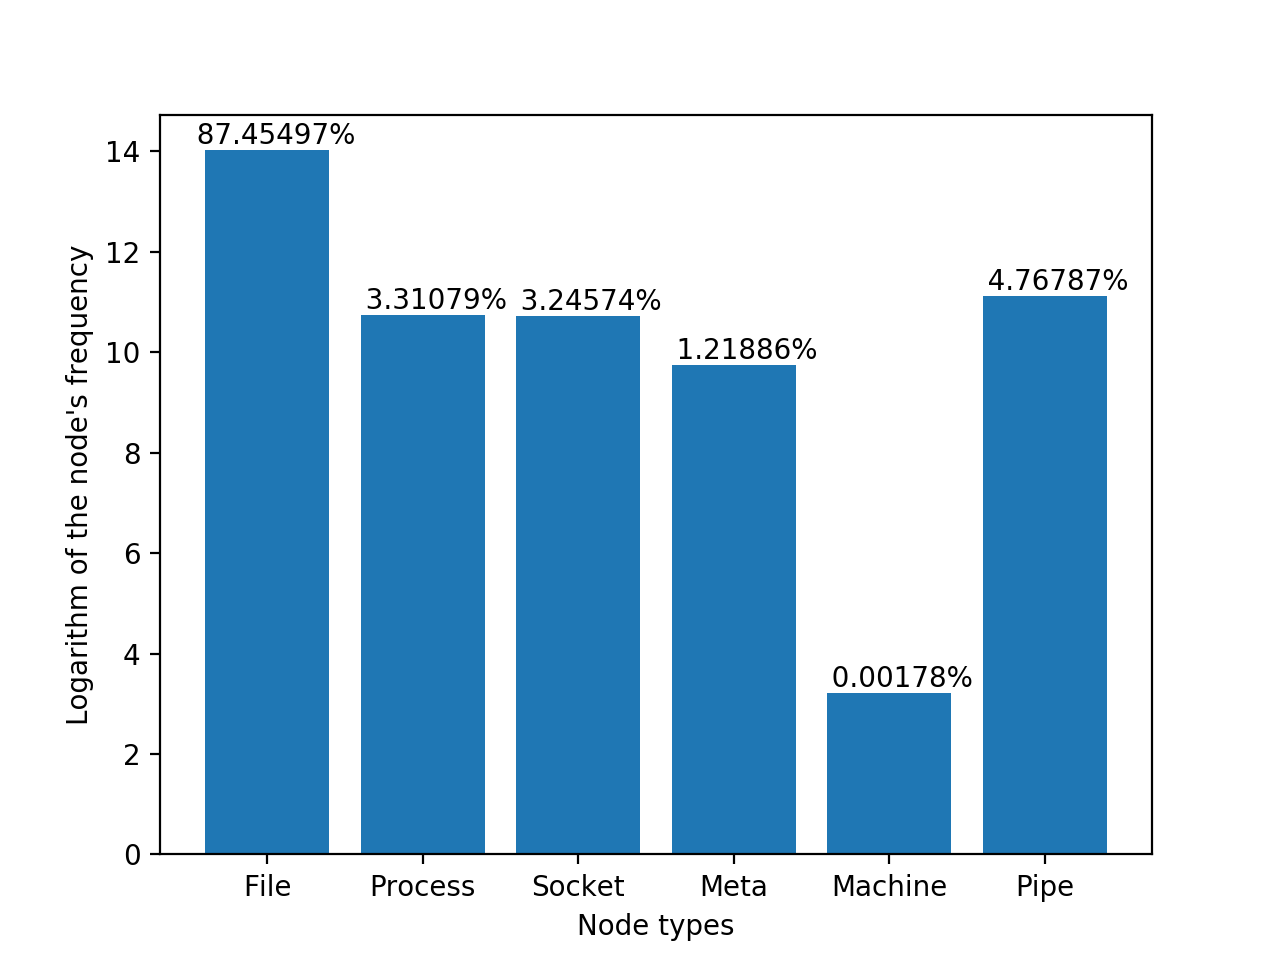
\includegraphics[width=0.7\textwidth]{graphics/node-freq-graph}
		\caption[\textbf{Log-scale node frequency}]{
			Bar chart above showing the log-scale node frequency in a database of $1,402,053$ nodes and $2,090,741$ edges. 
		}
		\label{Figure 2.1.1}
	\end{figure}
	Relationships between nodes are illustrated by different types of edges. Some edges also illustrate how an object (File, Socket, etc.) evolves over time. This is done using the \textit{GLOB\_OBJ\_PREV} edge and helps us to easily visualize the different versions of an object.
	\begin{figure}[H]
		\centering

		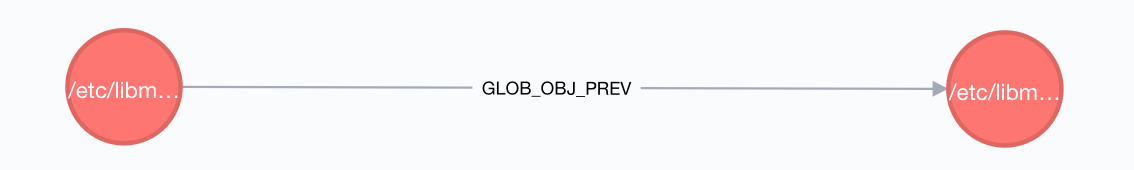
\includegraphics[width=0.7\textwidth]{graphics/GLOB_OBJ_PREV}
		\caption{
			Two versions of the same file connected via a GLOB\_OBJ\_PREV edge.
		}
		\label{Figure 2.1.2}
	\end{figure}
	A number of the edge types also use a \textit{state} field, in order to provide further information regarding the relationship between two nodes. For example, in the case of a \textit{PROC\_OBJ} edge connecting a File to a Process, the \textit{state} field is used to show whether the Process reads/ writes to the File or if the File is the binary the Process is executed from. \textit{PROC\_OBJ} edges also connect Processes to Sockets. Here, the \textit{state} field can take values such as: \textit{Server} (if the Process uses the Socket to accept new connections), \textit{Client} (if the Process uses to Socket to connect to a different Process that acts as a server - which may or may not be on a different machine)  and \textit{RaW} (if the Process also reads and writes through the Socket).
	\begin{figure}[H]
		\centering
		
		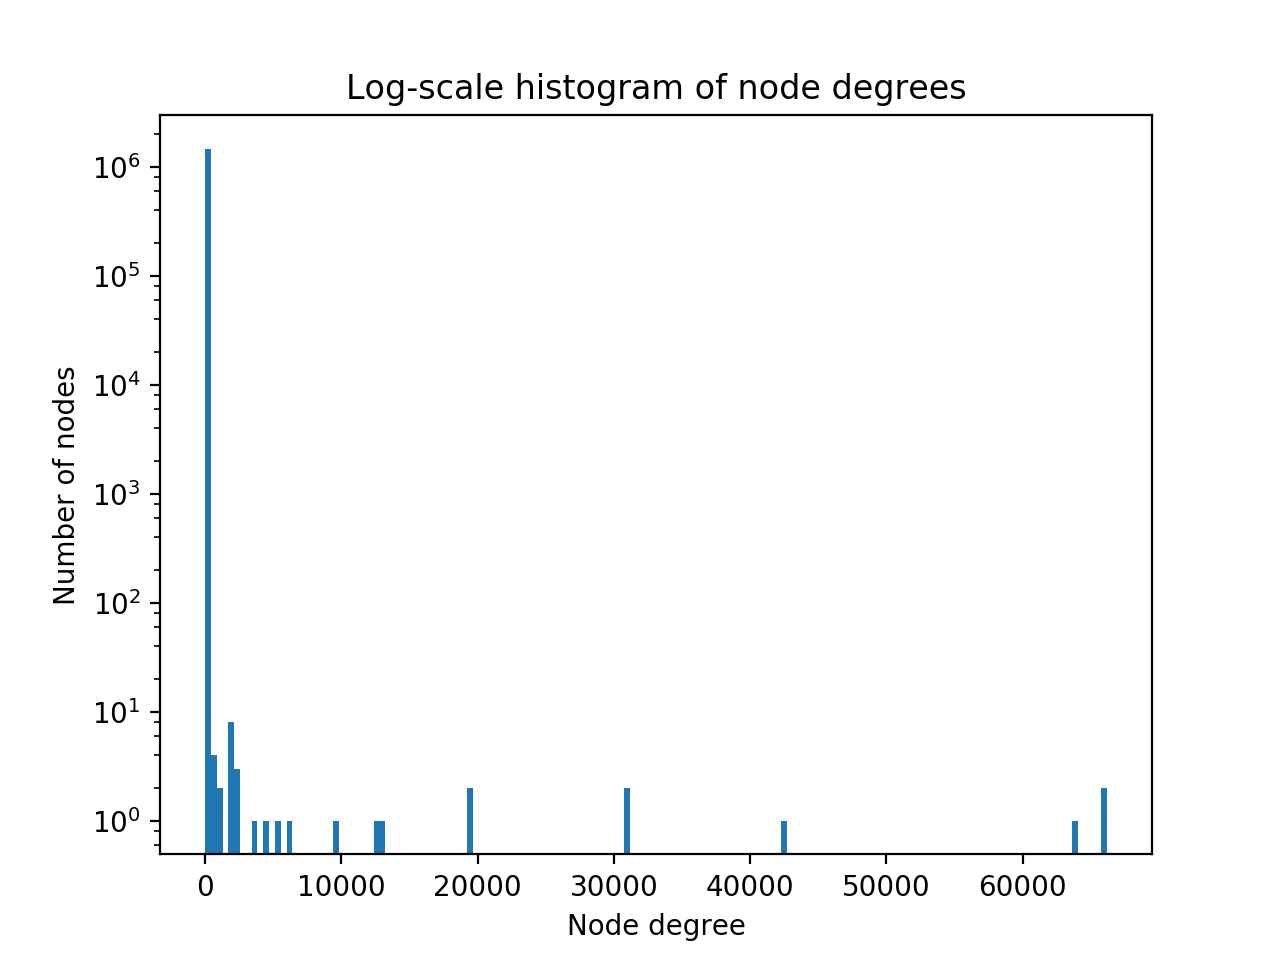
\includegraphics[width=0.7\textwidth]{graphics/node_degree_hist}
		\caption[Log-scale distribution of node degrees]{
			Log-scale histogram showing the distribution of node degrees, using the same graph as the one from Figure \ref{Figure 2.1.1} as source(i.e. $1,402,053$ nodes and $2,090,741$ edges).
		}
		\label{Figure 2.1.3}
	\end{figure}
	 
	 The graphs resulting from tracing are very sparse, with a number of edges almost equal to the number of nodes. This observation is also sustained by the histogram in Figure \ref{Figure 2.1.3}, where we can observe that most of the nodes have degrees between 0 and 10, while there also are a few nodes with a very high degree (up to $60, 000$). Therefore, the degrees of the nodes encountered in the database follow a power-law distribution\cite{Clauset:2009:PDE:1655787.1655789}.
	 
	\subsection{Ground truths} \label{Section: prep/data/ground-truths}
	In order to apply appropriate supervised learning algorithms, I had to build a labelled dataset of nodes from the raw data stored in graph format. This required setting a number of \textit{ground truths} of what a node of interest is. 
	\\ \\
	These ground truths are represented by a set of 6 rules, where I took into consideration a subset of node types: Files, Processes and Sockets. The rules are:
	\begin{enumerate}
		
		\item \textbf{Sockets that connect to an external IP: }Any socket that connects to an IP address other than 127.0.0.1 (localhost) can be considered a possible security breach because it could be used to leak information.
		
		\item \textbf{Files downloaded from the web and then executed: }Any file downloaded from the web can be suspicious, because we can not trust the source. Especially if it is executed, it can pose a real security threat to the system. The graph representation in the Neo4J database can be seen in Figure \ref{Figure 2.3}.
		\begin{figure}[H]
			\centering
			\includegraphics[width=0.7\textwidth]{graphics/downloaded-and-executed}
			\label{Figure 2.3}
			\caption{Graph representation of a file downloaded and then executed}
		\end{figure}
		In the figure above, Process1 writes the File while it is connected to the Socket and then Process2 starts, using File as binary.
		
		\item \textbf{File read from/ written to by a Processes that also opens a Socket to a different machine: }Here are two cases we need to treat separately. If the Process reads from the File, we face a potential leak of the File's contents. If the Process writes to the File, on the other hand, it might be the case that it corrupts its contents. This is a potential threat especially if the File is a sensitive file of the operating system (e.g. any file in /lib/ or /bin/). 
		
		\item \textbf{Processes that open a Socket to a different machine: }As mentioned at point 1, any Socket connecting to an external machine is a potential threat. In the same time, any process that opens a Socket to a different machine can be a source of suspicious behaviour, as well. 
		
		\item \textbf{Processes that runs suspicious commands: }Here, I define the term of \textit{suspicious command} as being one of the following bash commands:
		\begin{itemize}
			\item \textit{sudo} - gives the user running the Process root privilege. An attacker might use this to access OS-sensitive locations (such as /bin or /lib). 
			\item \textit{usermod/ groupmod} - an attacker might make use of these commands to change the running user's privileges and access files that it wouldn't otherwise have access to.
			\item \textit{chmod} - an attacker might use this command to change the access control to a specific File in order to make it accessible from external sources.
			\item \textit{rm -rf} - an ill-intended user might use this command to delete files crucial to the system. 
		\end{itemize}
	
		\item \textbf{Processes that writes to files in suspicious locations: }Here, I define the term of \textit{suspicious location} as being a location that is essential to the running of the system. These locations include:  \textit{/bin, /etc, /lib, /usr/bin, /usr/lib, /boot, /root, /dev, /etc/pwd}.
	\end{enumerate}
	These rules only represent a suitable starting point for the tool implemented here. In practice, though, I would expect my model to be driven by past analyst observations and interactions in the UI. This is a fact I kept in mind when considering various machine learning models, in order to try to create ones that can be updated given analyst input.
	\\ \\
	By setting these ground-truths, this project is also exploring whether the various machine learning algorithms implemented as part of this project can easily learn a number of patterns in the same time.
	\subsection{Data preprocessing} \label{Section: prep/data/feature-vectors}
	The implemented machine learning models only look at 3 of the 6 types of nodes: \textbf{File}, \textbf{Process} and \textbf{Socket} nodes. 
	\\ \\
	In order to achieve this, I had to define a set of features that would construct the \textit{feature vectors} representing each node. Furthermore, for graph-specific models (such as Graph Attention Networks) I also built the adjacency matrix of the given graph. 
	\\ \\
	I defined 13 features that would describe each node, in the same time taking into account its 'neighbour'. For a Process, the neighbour is the closest File or Socket connected to it. Here, \textit{'the closest node'} is the node that with the closest timestamp to it. Similarly, for a File or Socket, the neighbour is the closest Process node connected to it. Out of these 13 features, 3 are categorical (such as the type of node in question), 6 are binary (i.e. taking a True/ False value), 3 are integers (e.g: the version number of the node) and one is real (the base 2 logarithm of the distance in epochs to the node's neighbour). Appendix \ref{Appendix: Feature-vector} breaks down these features and explains the reasoning behind them in detail. When using one-hot-encoding for the 3 categorical features, the feature vectors increase their length to 23.

	\section{Machine learning models} \label{Section 2.2}
	This section describes the underlying theory of the machine learning models explored as part of this project and how they can be applied to the data I am working on.

	\subsection{Supervised learning using neural networks} \label{Section 2.2.2}
	Given a training sequence $\mathbf{s} = [(\mathbf{x_1}, y_1), (\mathbf{x_2}, y_2) \dots (\mathbf{x_m}, y_m)]$, a neural network learns a hypothesis $h: \mathbb{R}^n \rightarrow \mathcal{C}$ that maps an input feature vector $\mathbf{x}$ to its corresponding label $y$. 
	\\ \\ 
	The hypothesis is set as $h(\mathbf{x}) = f(\mathbf{x}; \mathbf{w}, \mathbf{b})$, where $f$ is a function dependent on the neural network architecture and $\mathbf{w}$ and $\mathbf{b}$ are the weights and biases, respectively. 
	\\ \\
	A \textbf{loss function} is usually defined to measure some notion of the neural network's error when estimating $y$ from $\mathbf{x}$, given $\mathbf{w}$ and $\mathbf{b}$. The training step involves an optimisation algorithm which aims at finding $\mathbf{w}$ and $\mathbf{b}$ such that the loss function is minimized. 
	
 	\subsubsection{Multilayer perceptron}  \label{Section 2.2.2.2}
	Neural network architectures consist of multiple interconnected artificial neurons in order to infer complex functions. The mutilayer perceptron (MLP) represents a class of feedforward artificial neural networks (ANN) where the neurons are arranged in three or more layers (as shown in Figure \ref{Fig: prep/ml/mlp/mlp}). MLPs are \textbf{fully connected}; that is each neuron in one layer connects to every neuron in the following layer with a certain weight $w_{i, j}$

	\begin{figure}[H]
		\centering
		\includegraphics[width=0.7\textwidth]{graphics/nns/multilayer}
		\caption[Multilayer perceptron]{
			Figure showing a 2-layer neural network.
		}
		\label{Fig: prep/ml/mlp/mlp}	
	\end{figure}	

	 Each layer of the MLP consists of a number of neurons(Figure \ref{Fig: prep/ml/mlp/neuron}). For an input vector $\mathbf{x}\in\mathbb{R}^d$, a weight vector $\mathbf{w}\in\mathbb{R}^d$, and a biast $b$, a neuron computes the output $y = \sigma(b + \sum_{i=1}^{d} w_i x_i)$, where $\sigma$ is an \textit{activation function}.
	
	\begin{figure}[H]
		\centering
		
		\includegraphics[width=0.7\textwidth]{graphics/nns/single_neuron}
		\caption[\textbf{Artificial neuron}]{
			Figure showing a single artificial neuron. 
		}
		\label{Fig: prep/ml/mlp/neuron}
	\end{figure}
	\subsubsection*{Activation functions}
	The main purpose of using an activation function $\sigma$ is to map the output of the linear combination of input features onto a desired (finite) range. Moreover, choosing the appropriate activation function can speed up the training process and even help us avoid the overfitting problem. Some frequently encountered activations functions are:
	\begin{enumerate}
		\item the \textbf{linear function}
		\begin{equation}
		\sigma(x) = cx 
		\end{equation}
		where $c \in \mathbb{R}$ is a constant. 
		
		\item the \textbf{sigmoid function}
		\begin{equation}
		\sigma(x) = \frac{1}{1+e^{-x}}
		\end{equation}
		
		\item the \textbf{tanh function}
		\begin{equation}
		\sigma(x) = \tanh(x) = \frac{2}{1+e^{-2x}} - 1
		\end{equation}
		Essentially, the $\tanh$ function is a scaled sigmoid function. It can be re-written as: $\tanh(x) = 2 \times \text{sigmoid}(2x) - 1$ 
		
		\item the \textbf{rectified linear unit (ReLU) function}
		\begin{equation}
		\sigma(x) = 
		\begin{cases}
		0 & \text{if } x < 0 \\
		x & \text{if } x \geq 0
		\end{cases}
		\end{equation}
		
		\item the \textbf{leaky rectified linear unit (LReLU) function}
		\begin{equation}
		\sigma(x) = 
		\begin{cases}
		0.001x & \text{if } x < 0 \\
		x & \text{if } x \geq 0
		\end{cases}
		\end{equation}
	\end{enumerate} 
	In the past, the $\tanh$ used to be the activation function of choice in neural networks, but recent works\cite{nonlinearities} have shown that rectified nonlinearities (such as ReLU or LReLU) considerably improve the performance of the model. Figure \ref{Fig: prep/ml/mlp/activations} shows the graphs of three of the activation functions above ($\tanh$, ReLU and LReLU) and their derivatives.
	\begin{figure}[H]
		\centering
		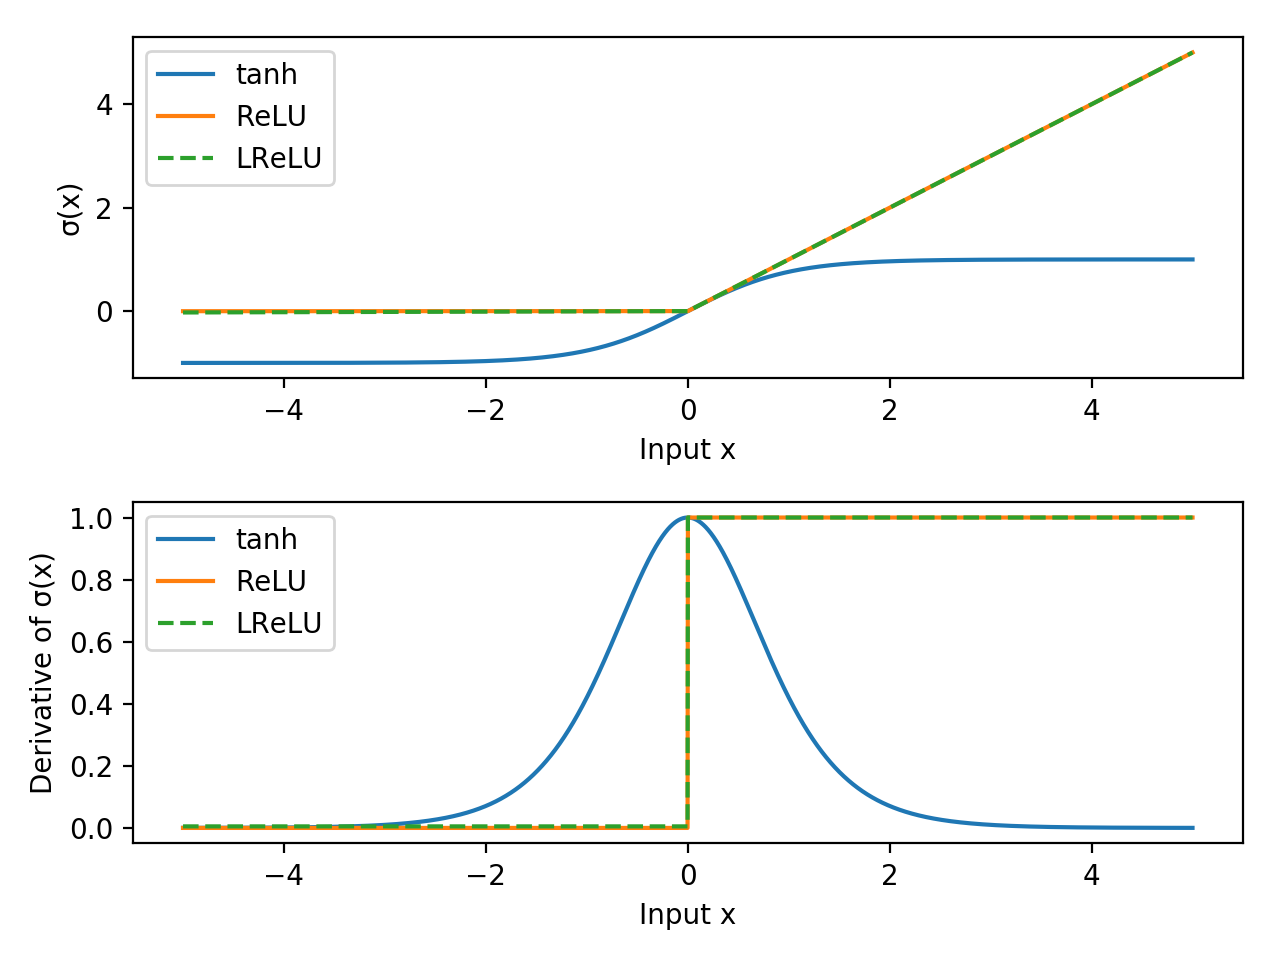
\includegraphics[width=0.7\textwidth]{graphics/nns/activations}
		
		\caption[Activation functions]{The $\tanh$, ReLU and LReLU functions and their derivatives}
		\label{Fig: prep/ml/mlp/activations}
	\end{figure}
	In general, neural networks are optimised using gradient-based algorithms. Therefore, activation functions with steeper gradients (such as ReLU and LReLU) tend to make the algorithm to converge faster.
	
	\subsubsection*{Using MLPs for classification}
	In this project, I intend to classify nodes as being in one of two classes: \textit{SHOW} and \textit{HIDE}, based on the feature vectors described in Section \ref{Section: prep/data/feature-vectors}. Therefore, we are interested in seeing how an MLP can be used to solve classification problems. As shown by Cybenko's theorem\cite{sigmoidal}, MLPs are universal function approximators, so that they can be used to create mathematical models by regression analysis. Considering the fact that classification is a particular case of regression where the response variable is categorical, we can infer that MLPs make good classifier algorithms. 
	\\ \\
	Suppose the MLP has to learn to classify a feature vector $\mathbf{x} \in \mathbb{R}^d$ into a class $C_t$ from $\mathcal{C} = \{C_1\dots C_k\}$. In this case, we want the $t^{th}$ output neuron (i.e. $o_t$) to indicate this. A popular choice for this task is the \textbf{softmax function}, which transforms any k-dimensional vector $\mathbf{o}$ to the probability distribution:
	\begin{equation}
		\centering
		\text{softmax}_i(\mathbf{o})_i = \frac{e^{o_i}}{\sum_{j=1}^{k}e^{o_j}}
	\end{equation}
	where: $\mathbf{o}^T = [o_1\dots o_k]$ is the vector of the output neurons. Thus, the probability of the input vector $\mathbf{x}$ being in class $C_t$ is given by:
	\begin{equation}
		\centering
		\begin{split}
			\mathbb{P}(y = C_t | \mathbf{x}) & = \text{softmax}_i(\mathbf{o})_t \\
			& = \frac{e^{o_t}}{\sum_{j=1}^{k}e^{o_j}}
		\end{split}
		\label{Eq: prep/ml/mlp/softmax}
	\end{equation} 
	
	If we consider the hidden layer from Figure \ref{Fig: prep/ml/mlp/mlp} to use the ReLU activation function, we can re-write the equation \ref{Eq: prep/ml/mlp/softmax} in vector format as follows: 
	\begin{equation}
		\centering
		\mathbb{P}(y=C_t | \mathbf{x}) = \frac
		{
			\exp (\mathbf{W_2}\text{ReLU}(\mathbf{W_1 x} + \mathbf{b_1}) + \mathbf{b_2})_t
		}
		{
			{\sum_{j=1}^{k}\exp (\mathbf{W_2}\text{ReLU}(\mathbf{W_1 x} + \mathbf{b_1}) + \mathbf{b_2})_j}
		} 
	\end{equation}
	
	where $\mathbf{x}$ is the input feature vector.
	
	\subsubsection*{Training the MLP}
	Using a training sequence $\mathbf{s}$, the parameters of the MLP have to be optimised in order to be able to have a performant classifier. One of the most frequently used optimisation techniques is \textbf{gradient descent}, which updates the parameters iteratively, by moving in the direction of the gradient of a loss function. In a complex system, the gradient is calculated using \textbf{backpropagation}. This algorithm is described in detail in Appendix \ref{appendix-MLP-opt}. 
	
	\subsection{Convolutional Neural Networks} 
	Classically, Convolutional Neural Networks(CNNs) are used in tasks such as computer vision or natural language processing. One-dimensional CNNs, though, have proven to be effective for non-spatial data, as well, by identifying relations between the features from the input feature vectors. For this reason, I considered this as a potential model in my project. 
	\\ \\
	CNN make use of \textbf{convolutional layers} in order to identify relations between features in a subarea of the feature vector. 	Following these convolutional layer(s), a CNN normally has a one or more fully connected layers that process the outputs and return either a probability distribution (for classification) or a single value (in the case of regression).  
	
	\subsubsection*{Convolutional layer}
	The main purpose of the convolutional layer is to extract relationships between the features from an input vector. It uses a fix-sized kernel $\mathbf{w} \in \mathbb{R}^k$, that slides over the input vector $\mathbf{x}\in\mathbb{R}^d$ and computes a linear transformation for every patch of size $k$. The output of the convolutional layer is a new vector $\mathbf{y}\in\mathbb{R}^n$, where $n=d - k + 1$. The values of each element in the output vector is given by the equation:
	\begin{equation}
		y_i = \mathbf{w}^T\mathbf{x}_{i:i+k-1}
	\end{equation}
	where $\mathbf{x}_{a:b}$ represents the sub-vector containing all elements $x_i. \forall a\leq i \geq b$. Figure \ref{Fig: prep/ml/cnn/convoLayer} shows the step-by-step construction of the output vector.
	\begin{figure}[H]
		\centering
		\begin{subfigure}[b]{0.3\linewidth}
			\includegraphics[width=\linewidth]{graphics/nns/conv/1}
			\vspace*{1cm}
		\end{subfigure}
		\begin{subfigure}[b]{0.3\linewidth}
			\includegraphics[width=\linewidth]{graphics/nns/conv/2}
			\vspace*{1cm}
		\end{subfigure}
		\begin{subfigure}[b]{0.3\linewidth}
			\includegraphics[width=\linewidth]{graphics/nns/conv/3}
			\vspace*{1cm}
		\end{subfigure}
		\begin{subfigure}[b]{0.3\linewidth}
			\includegraphics[width=\linewidth]{graphics/nns/conv/4}
		\end{subfigure}
		\begin{subfigure}[b]{0.3\linewidth}
			\includegraphics[width=\linewidth]{graphics/nns/conv/5}
		\end{subfigure}
		\begin{subfigure}[b]{0.3\linewidth}
			\includegraphics[width=\linewidth]{graphics/nns/conv/6}
		\end{subfigure}
		\caption[1D Convolution]{Step-by-step example of 1D convolution with a $1\times3$ kernel}
		\label{Fig: prep/ml/cnn/convoLayer}
	\end{figure}
	In order to add further nonlinearity and prevent the overfitting of the model, one may also use an activation function $\sigma$ when computing the final outputs of the layer. Furthermore, in order to manipulate the length of the output vector, we can also use \textbf{zero-padding}, which simply pads the input vector with zeros, such that the output preserves its length.
	\\ \\
	\textbf{Dilated convolution}(Figure \ref{Fig: prep/ml/cnn/dilated}) is a technique that increases the receptive (global) view of the network exponentially and has proven extremely effective in tasks such as context and text-to-speech resolution. In this case, the filter (kernel) is applied over a larger area than its length by skipping input values with a certain step, called \textit{dilation field}. Exponentially increasing the dilation rate results in an exponential field growth in depth\cite{DBLP:journals/corr/YuK15}.  
	\\ \\
	Recent work has shown that dilated convolution is a simple by effective idea when it comes to detection of fine-grained details by processing inputs in higher resolutions. For this reason, I have considered applying this approach to the problem at hand.
	
	\begin{figure}[H]
		\centering
		\includegraphics[width=.8\textwidth]{graphics/nns/conv/dilated}
		\caption[Dilated convolution]{Dilated convolution schema reproduced from \textit{van den Oord et al.} \citep{DBLP:journals/corr/OordDZSVGKSK16}}
		\label{Fig: prep/ml/cnn/dilated}
	\end{figure}
	
	\subsubsection{Probabilistic Neural Networks}
 	Probabilistic Neural Networks (PNNs) are non-parametric classifiers that try to assign a class to an input pattern based on the pre-estimated probability density function of each class. Suppose we want to classify n-dimensional vectors $\mathbf{x} \in \mathbb{R}^n$ into one of $k$ classes in $\mathcal{C}=\{C_1\dots C_k\}$. Based on a training sequence $\mathbf{s} = \{ (\mathbf{x}_1, C), (\mathbf{x}_2, C), \dots ,(\mathbf{x}_m, C)\}$ we estimate the probability density functions $p_i(\mathbf{x}). \forall i \in \{1,2,\dots,k \}$ for every class in $\mathcal{C}$. 

  	\begin{figure}[H]
 		\centering
 		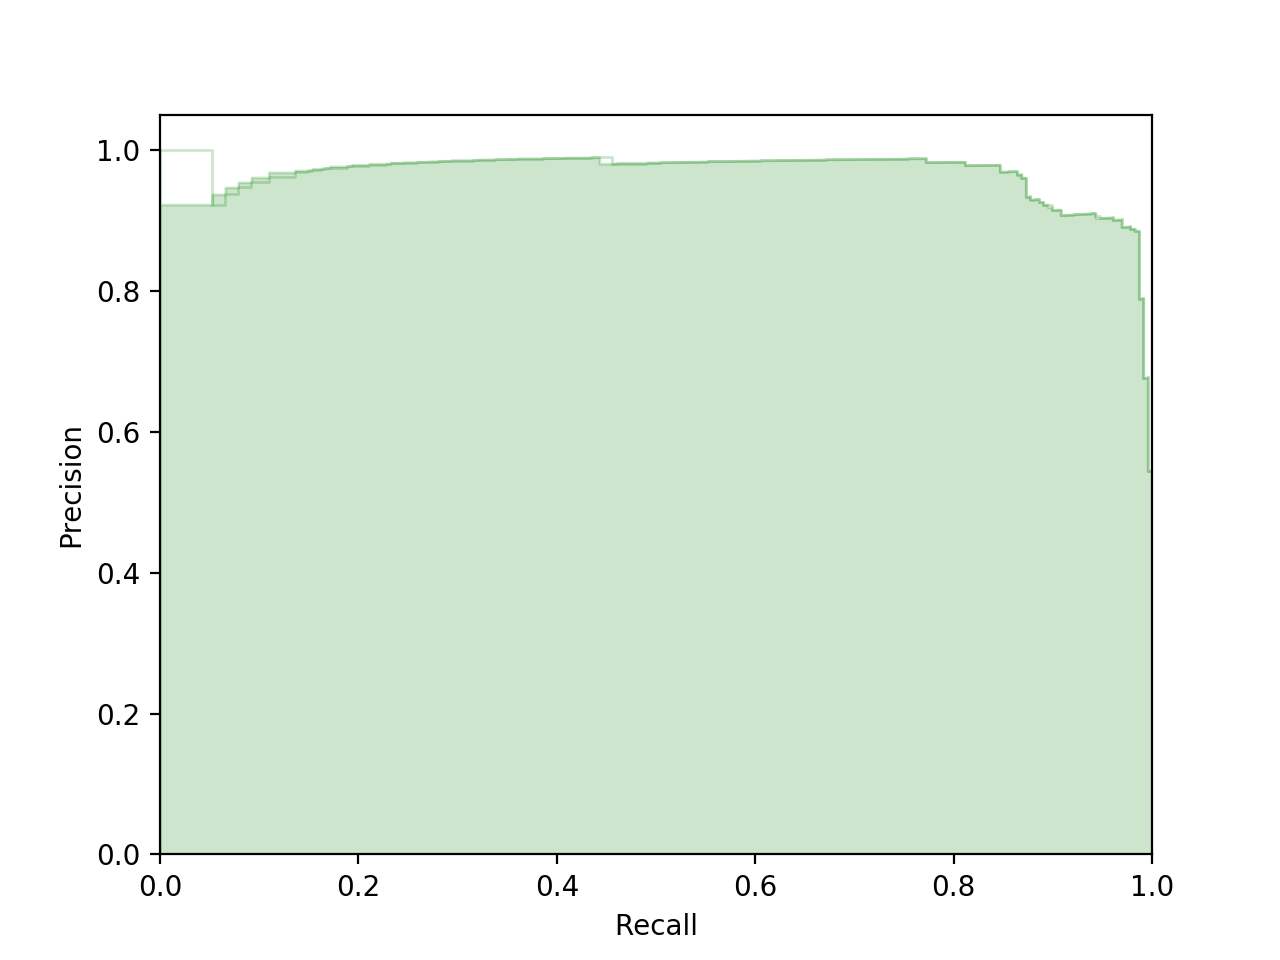
\includegraphics[width=\textwidth]{graphics/nns/pnn}
 		\caption{PNN architecture}
 		\label{Fig 2.8}
 	\end{figure}
	 
	 Figure \ref{Fig 2.8} shows a general-purpose PNN architecture that can be used for classification. It consists of $n$ input units, $m$ pattern units and $k$ output units. Each pattern unit forms the inner product of its weight vector $\mathbf{w}$ and the normalized pattern vector $\mathbf{x}$ and outputs $\exp(\frac{\mathbf{w}^T\mathbf{x} - 1}{\sigma^2})$. Each category unit sums up the outputs of the pattern units connected to it. This insures that the activity in each of the category units represents the Parzen-window density estimate using a circular symmetric Gaussian window of covariance $\sigma^2\mathbf{I}$, where $\mathbf{I}$ is the $n\times n$ identity matrix. $\sigma$ is a parameter set by the user and is equal to $\sqrt{2}$ times the width of the effective Gaussian window
     \\ \\ 
	 The weights of the $p^\text{th}$ pattern unit are set as $\mathbf{w}_p = \mathbf{x}_p$, $\forall p \in \{ 1,2,\dots ,m \}$, where $\mathbf{x}_p$ is the normalised $p^\text{th}$ pattern from the training set. In order to classify the a new normalized pattern $\mathbf{x}$ we first have to propagate the it through the network. Then, the resulting class will be $C_t$, where:
	 \begin{equation}
		 t = \argmax_i c_i(\mathbf{x}). \forall i \in \{1,\dots k\}
	 \end{equation}
	 and $c_i(\mathbf{x})$ is the output of the $i^\text{th}$ category unit.
	\section{API architecture} \label{Section 2.3}
	Once I decided how to pre-process the raw graph data and researched different applicable machine learning models, I looked into solutions to facilitate interaction between the CADETS user interface and the classifiers. It is desirable for the filtering tool and the UI to be decoupled, in order to allow independent evolution of both parties without affecting the other. For this reason, I decided to use a \textit{\textbf{Representational State Transfer (REST) API}}, taking advantage of the HTTP protocol to facilitate communications with the user interface.
	\\ \\
	Unlike other similar protocols such as SOAP or RPC, REST APIs are not constrained to a single communications format and are do not impose any specific parameters order, therefore providing flexibility. REST APIs are stateless, allowing each call to be made independently, containing solely the data necessary to complete itself successfully. Moreover, the different layers involved in a REST APIs' architecture make it highly modular and scalable. 
	\\ \\
	Being stateless, a REST API might increase the per-request overhead significantly by having to handle loads of incoming and outbound calls. Therefore, it is essential that it is designed to encourage the caching of intermediate results.
	
	\section{Requirements analysis} \label{Section 2.4}
	Having reviewed the structure of the raw graph data, the background theory of the machine learning models and the structure that will facilitate interaction with the CADETS user interface, the requirements of the project overall were closely examined. The end goal of this project is to have an independent and modular tool that is able to connect to the CADETS UI and efficiently classify the nodes from a given graph. A breakdown of the project requirements can be visualized in Table \ref{Table 2.2}.
	\begin{longtable}{|p{.51\textwidth}|p{.13\textwidth} p{.13\textwidth} p{.13\textwidth}|}
		\textbf{Requirements} & \textbf{Priority} & \textbf{Risk} & \textbf{Difficulty} \\
		\hline
		Implementation of baseline model & High & Low & Low \\
		MLP Implementation & High & Medium & Medium \\
		Implementation of CNN & Medium & High & Medium \\
		PNN Implementation & Medium & Medium & High \\
		Implementation of the server infrastructure & High & Medium & Medium \\
		Server-side caching implementation for previous results & Medium & Low & Low \\
		Comparative evaluation of the implemented machine learning models & High & Medium & High \\
		\hline
		\caption[Requirements overview]{\centering Overview of the high-level requirements, their priorities, risks and difficulties.}
		\label{Table 2.2}
	\end{longtable}
	\section{Choice of tools} \label{Section 2.5}
	This section describes the tools choices that I made in order to meet the requirements described in Section \ref{Section 2.4}. 
	\subsection{Programming languages} \label{Section 2.5.1}
	Early in the planning stage I decided to use Python 3.6.4\footnote{\textbf{\url{https://www.python.org/downloads/release/python-364/}}} as the main programming language. It is extremely popular in both research and industry deep learning communities, providing a large variety of libraries that can be utilised to this end. 
	\\ \\
	Besides Python, I also used the Cypher Data Manipulation Language (DML) in order to interact to the original graph data stored in Neo4J.  
	
	\subsection{Libraries} \label{Section 2.5.2}
	Apart from the Python built-in libraries, I also used the third-party libraries described in Table \ref{Table 2.3}. 
	\begin{longtable}{|p{.15\textwidth} p{.10\textwidth} p{.4\textwidth} p{.25\textwidth}|}
		\textbf{Library} & \textbf{Version} & \textbf{Purpose} & \textbf{Licence}\\
		\hline
		keras & 2.1.5 & Building and running the neural networks. & MIT Licence \\
		numpy & 1.14.2 & Efficient mathematical operations on vectors and matrices. High precision floating-point calculations. & NumPy Licence\\
		scipy & 1.0.0 & Processing frames and evaluating the machine learning models. & SciPy Licence\\
		pandas & 0.22.0 & Working with tabular data-structures & BSD 3-Clause Licence\\
		flask & 0.12 & Handling the HTTP requests in the REST API layer. & BSD 3-Clause Licence\\
		matplotlib & 2.0.0 & Plotting graphs. & PSF Licence \\
		neo4j-driver & 1.5.3 & Querying the Neo4J database. & Apache 2.0 Licence\\
		pymongo & 3.6.1 & Handling the server-side caching of classification results. & Apache 2.0 Licence\\
		\hline
		\caption[Libaries table]{\centering Table showing the third-party libraries used  as part of this project}
		\label{Table 2.3}
	\end{longtable} 
	The library of key importance to the project is \textbf{Keras}, a high-level neural networks API using Tensorflow\footnote{\textbf{\url{https://www.tensorflow.org/}}} as backend. It is a modular and easily extensible library that fits the iterative software development methodology adopted in this project.
	\subsection{Development and testing environment}
	Development work was entirely done on my personal machine -- a 15" Macbook Pro, running MacOS High Sierra (version 10.13.2). The IDE I chose for this project was \textbf{PyCharm}\footnote{\textbf{\url{https://www.jetbrains.com/pycharm/}}}, due to its high flexibility and support for version control and testing.
	\\ \\
	For a project at this scale, version control is crucial. In order to organize my codebase accordingly, I used the \textbf{git} version control environment and synchronized it remotely with the free online hosting service \textit{GitHub}\footnote{\textbf{\url{https://github.com}}}. GitHub was also used as the main backup strategy for this project.
	\\ \\
	A separate GitHub repository was used to maintain the \LaTeX \space code for this dissertation. 
	
	\section{Starting point} \label{Section 2.6}
	At the start of this project, I had intermediate knowledge of Python, having used it in the Part 1B group project and a number of other small personal projects. However, having had no previous experience with Keras, I had to become acquainted with the API and to learn how to use it to configure neural networks.   
	\\ \\
	In terms of theoretical background, the Artificial Intelligence I course provided sufficient initial knowledge to understand the high-level behaviour of MLPs. Additional research was required to understand the CNNs and non-parametric techniques implemented. The full list of Tripos courses that were applicable to the project can be seen in Table \ref{Table 2.4}.
	
	\begin{longtable}{|p{.40\textwidth} | p{.50\textwidth}|}
		\textbf{Course} & \textbf{Applicability} \\ 
		\hline
		Artificial Intelligence I & Basic machine learning and neural networks \\
		Databases & Interacting with the Neo4J database \\
		Concurrent \& Distributed Systems & REST API setup \\ 
		Networking & Handling HTTP requests \\
		Operating Systems & High-level understanding of UNIX-based operating systems\\
		Security I & Basic notions of UNIX security setup \\
		\hline
		\caption[Computer Science Tripos courses and their applicability to this project.]{\centering Computer Science Tripos courses and their applicability to this project.}
		\label{Table 2.4}
	\end{longtable}
	
	\section{Software engineering techniques} \label{Section 2.7}
	For the purpose of this project, I decided to use the \textbf{Iterative and Incremental Development Model}. I divided the overall project into three separate modules: 
	\begin{enumerate}
		\item An \textit{interface that communicates with the Neo4J database} in order to extract the features vectors that are used by the machine learning models.
		\item The actual \textit{machine learning models}. 	An initial implementation was developed for each model, which was iteratively refined in order to improve its performance.  
		\item The \textit{server interface} that would handle requests from the CADETS client.
	\end{enumerate}

	\section{Summary} \label{Section 2.8}
	In this chapter I discussed the data the machine learning models work on and how it is preprocessed, the background theory that had to be understood and the software engineering decision that were made before the work could begin. I have presented a condensed theory of the models that were implemented as part of this project. I have also described how the machine learning models will interact with the external sources (i.e. the Neo4J database and the CADETS UI).
	\\ \\
	The next chapter will provide a detailed breakdown of the implementation, showing how the aims described here were accomplished. 
	
\end{document}

%%%%%%%%%%%%%%%%%%%%%%%%%%%%%%%%%%%%
%%%%%%%%%%%%  IMPLEMENTATION %%%%%%%%%%%
%%%%%%%%%%%%%%%%%%%%%%%%%%%%%%%%%%%%
\begin{document}
	\chapter{Implementation}
	This chapter describes the describes how the requirements described in the previous chapter have been accomplished. 
	\section{Overall structure of the project} \label{Section: impl/overview}
	The main objective I had while implementing the project was to be able to have a completely independent tool that is can communicate with the CADETS client and classify nodes successfully. In order to achieve this, I divided the overall project into three smaller sub-modules:
	
	\begin{enumerate}
		\item \label{impl/overview/enum/1} The \textbf{Neo4J interface}, which handles the interaction between my tool and the Neo4J database that stores the raw graph data with the end purpose of extracting the nodes' feature vectors. This is described in detail in Section \ref{Section: impl/neo4j}.
		\item The \textbf{machine learning models}, which use the feature vectors extracted as part of the \ref{impl/overview/enum/1}$^{\text{st}}$ module in order to classify the nodes into \textit{SHOW} or \textit{HIDE}. The exact details of how they were implemented in Section \ref{Section: impl/ml}.
		\item The \textbf{REST API}, which wraps around the previous two modules and handles requests received by the tool. This is described in detail in Section \ref{Section: impl/REST}.
	\end{enumerate}
	Figure \ref{Fig: impl/pipeline} shows a schema of how the 3 modules will work together as a part of a request processing pipeline. 
	\\ \\
	In the following sections, I will describe the modules listed above in a bottom-up approach -- from the Neo4J interaction to the REST API. 
	\begin{figure}[H]
		\centering
		\includegraphics[width=.95\textwidth]{graphics/overall-schema}	
		\caption[Processing pipeline]{Overview of the project's processing pipeline.}
		\label{Fig: impl/pipeline}
	\end{figure}
	\section{Neo4J interaction} \label{Section: impl/neo4j}
	This section describes how the project I implemented interacts with the Neo4J database and how the features for every node are extracted. 
	\subsection{Database driver} \label{Section: impl/neo4j/driver}
	The biggest challenge when designing the database driver was the choice of the library I would use to run the actual queries. There are a number of Python libraries available, out of which I took two into consideration: \textbf{py2neo}\footnote{\textbf{\url{http://py2neo.org/v3/}}} and \textbf{neo4j-driver}\footnote{\textbf{\url{https://github.com/neo4j/neo4j-python-driver}}}. In order to decide which one I will use, I timed the running of two queries(\textit{match (n) return n} and \textit{match(n) return n limit 1} ) and the overall feature extraction for one node on a database of $631, 357 \text{ nodes}$ for both libraries. The resulting times are shown in Table \ref{Table: impl/neo4j-driver-timings}:
	\begin{longtable}{|p{.15\textwidth}|p{.30\textwidth}p{.25\textwidth}p{.25\textwidth}|}
		\textbf{library} & \textbf{\textit{match(n) return n}} & \textbf{\textit{match(n) return n limit 1}} & \textbf{feature extraction} \\
		\hline
		\textit{py2neo} & $337.477\text{s } (\approx5.5 \text{ minutes})$ & $13\text{ms}$ & TODO \\ 
		\textit{neo4j-driver} & $97.288\text{s }(\approx1.5 \text{ minutes})$ & $28\text{ms}$ & $68.78\text{s}$  \\
		\hline
		\caption[Neo4J libraries timings]{\centering Table showing the timings for the two libraries considered}
		\label{Table: impl/neo4j-driver-timings}
	\end{longtable}
	The main purpose of the database driver is to support feature extraction(detailed in Section \ref{Section: impl/neo4j/features}). Therefore, given the times in Table \ref{Table: impl/neo4j-driver-timings}, I decided to use \textbf{neo4j-driver}. On top of this library, I wrote a wrapper class, \textbf{DatabaseDriver}. 
	\subsection{Feature extractor} \label{Section: impl/neo4j/features}
	The feature extractor uses the DatabaseDriver described in the previous section in order to build the feature vectors for a list of nodes, just as described in Table \ref{Table: prep/features}. Therefore, the two classes will be in an association relationship (i.e. the FeatureExtractor has one instance of DatabaseDriver), as displayed in Figure \ref{Fig: impl/neo4j-driver-uml}.
	\\ \\
	Considering the fact that the machine learning models require purely real feature vectors to work, I decided to use \textbf{one-hot-encoding} for the categorical features. In other words, for every such feature, I generated one extra boolean column for each category. Only one of these columns can take the value 1 for each sample. Using this encoding led to an increase in the length of the feature vectors, from 13 to 23 variables. 
	\\ \\
	On top of extracting the feature matrix, this module also has support for generating the adjacency matrix of the nodes from the list provided. This is required for models such as the Graph Attention Networks (Section \ref{Section: impl/ml/gat}).
	\begin{figure}[H]
		\centering
		\includegraphics[width=.5\textwidth]{graphics/umls/uml-neo4j-driver}
		\caption[FeatureExtractor UML class diagram]{\centering UML class diagram showing the interaction between the feature extractor and the database driver.}
		\label{Fig: impl/neo4j-driver-uml}
	\end{figure}
	\section{Machine learning models} \label{Section: impl/ml}
	With the first module being implemented, I started to implement different machine learning models that I would use to classify the nodes. 
	\subsection{Training set} \label{Section: impl/ml/training-set}
	One of the key requirements for a well-behaved machine learning model is to have a comprehensive training set. Keeping this in mind, I used the ground-truths listed in Section \ref{Section: prep/data/ground-truths} with the aim of extracting examples of nodes from both classes (i.e. \textit{SHOW} and \textit{HIDE}) from a database of $6,007$ nodes, out of which $5,498$ are of interest (i.e. either \textit{File}, \textit{Process} or \textit{Socket}). For all these selected nodes, I used the feature extractor in order to build a labelled training set $\mathbf{s}=\{ (\mathbf{x}_1, \mathbf{y_1}), \dots, (\mathbf{x}_n, \mathbf{y_n}) \}$ that will be used by all the models in the training phase. As expected, there is a significant imbalance in the training data, with $2,382$ nodes ($43.33\%$) being labelled as \textit{SHOW} and $3,115$ ($56.67\%$) being labelled as \textit{HIDE}. This is a factor that I took into consideration both when designing and evaluating the models.
	\\ \\
	Moreover, using the same training set for all the models implemented is one of the key factors that ensure the correctness of the models' comparative evaluation. 
	\subsection{Graph Attention Network} \label{Section: impl/ml/gat}
	\begin{figure}[H]
		\centering
		\includegraphics[width=.7\textwidth]{graphics/nns/gat}	
		\caption[Attention mechanism]{The attention mechanism computing the attention coefficients \\ $\alpha_{i,j}=\text{softmax}_j(a(\mathbf{Wh}_i, \mathbf{Wh}_j))$, where $a$ is the Leaky ReLU (LReLU) activation function, parametrized by a weight vector $\mathbf{a}\in\mathbb{R}^{2F'}$, namely: \\  $a(\mathbf{Wh}_i, \mathbf{Wh}_j)=\text{LReLU}(\mathbf{a}^T[\mathbf{Wh}_i\mid\mid\mathbf{Wh}_j])$}.
		\label{Fig: impl/attn-mechanism}
	\end{figure}
	\subsection{Probabilistic Neural Networks} \label{Section: impl/ml/pnn}
	The implementation of Probabilistic Neural Networks (PNNs) consisted of two steps: PNN training and classification. 
	\begin{algorithm}[H]
		\caption{PNN training}
		\begin{algorithmic}
			\Procedure{train\_PNN}{}
				\State $j \gets 0$
				\State $n \gets \text{number of patterns}$ 
				\Do
					\State $j \gets j + 1$
					\State $x_{jk} \gets \frac{x_{jk}}{\sqrt{\sum_{i=1}^{d}x_{ij}^2}}$ \Comment{\textbf{normalization}}
					\State $w_{jk} \gets x_{jk}$ \Comment{\textbf{training}}
					\If{$\mathbf{x} \in \omega_i$}
						\State $a_ic \gets 1$
					\EndIf
				\doWhile{$j \neq n$}
			\EndProcedure
		\end{algorithmic}
	\end{algorithm}
	\begin{algorithm}
	\caption{PNN classification}
	\begin{algorithmic}[H]
		\Procedure{classify\_PNN}{$\mathbf{x}$}
		\State $k \gets 0$
		\State $n \gets \text{number of patterns}$ 
			\Do
				\State $k \gets k + 1$
				\State $z_k \gets \mathbf{w_k}^T\mathbf{x}$
				\If{$a_{kc} = 1$}
					\State $g_c \gets g_c + \exp(\frac{z_k - 1}{\sigma^2})$
				\EndIf
			\doWhile{$k \neq n$} 
		\State $class \gets \argmax_i g_i(\mathbf{x})$ \\
		\Return{class}
		\EndProcedure
	\end{algorithmic}
\end{algorithm}
	\section{REST API} \label{Section: impl/REST}
	This section describes how the REST API layer that eases the application's interaction with the CADETS user interface was implemented.
	\subsection{Actual REST API} \label{Section: impl/REST/actual}
	The main entry point to the REST API receives a POST HTTP request from the client, containing a JSON file with a list of nodes to classify. Each node in the list will be represented by a (\textit{uuid}, \textit{timestamp}) pair, which allows the tool to uniquely identify it in the Neo4J database. The API then initiates a 'job' that starts classifying the nodes in background and replies with a JSON containing its ID.
	\\ \\
	Using this job ID, the client can then query the API using an HTTP GET request and the API will reply with a different JSON containing two fields: \textit{"results"} and \textit{"status"}. The \textit{"results"} field contains the list of nodes that have been classified so far as part of the job in question. The \textit{"status"} field can take one of three values, depending on what the status of the job is: \textit{WAITING} means that it is idle, \textit{RUNNING} means that the job is still classifying nodes and therefore the results returned are partial (i.e. only for a subset of the nodes) and \textit{DONE} represents the fact that the job is finished and the returned classification results are for the entire set of nodes queried initially. 
	\\ \\
	I decided to implement this 2-step mechanism due to the fact that node classification can take a long time, especially when working with large databases. This way, the client sends one request and then can query the API at any time for the job status and partial or final classification results. Figure \ref{Fig: impl/REST/API-integrate} shows how these jobs work in relation with the other modules.
	\begin{figure}[H]
		\centering
		\includegraphics[width=.9\textwidth]{graphics/umls/full-system-uml}
		\caption[General UML diagram]{\centering UML diagram showing the integration of API's jobs with the previous two modules(i.e. feature extractor and machine learning models).}
		\label{Fig: impl/REST/API-integrate}
	\end{figure}
	Another key factor that I took into consideration is how the API will treat different types of nodes, given the fact that the machine learning models only apply to \textit{File}, \textit{Socket} and \textit{Process} nodes. Table \ref{Table: impl/REST/API-strategy} shows the strategies adopted by the API for different types of nodes.
	\begin{longtable}{|p{.15\textwidth}|p{.85\textwidth}|}
		\textbf{Node type} & \textbf{API strategy} \\
		\hline
		\textit{File} & \multirow{3}{*}{Return the classification result for the node.} \\
		\textit{Socket} & \\
		\textit{Process} & \\
		\hline
		\textit{Machine} & Only represents $0.00178\%$ of the total number of nodes, so consider classified as \textit{SHOW} by default. \\
		\hline
		\textit{Meta} & \multirow{2}{*}{Return the classification result for the \textit{Process} node that it is connected to.} \\
		\textit{Pipe} & \\
		\hline
		\caption{API strategy for different type of nodes}
		\label{Table: impl/REST/API-strategy}
 	\end{longtable}
 
	\subsection{Caching mechanism} \label{Section: impl/REST/caching}
	Due to the stateless nature of REST APIs, caching is a desirable feature in order to avoid a high load on the application. Moreover, an efficient caching mechanism is essential to support the 2-step format of the API described in Section \ref{Section: impl/REST/actual}. 
	\\ \\
	In order to handle caching, I am using a PostgreSQL database, for its object-relational format. Unlike other SQL dialects (such as MySQL), it is highly customizable, providing stored procedures in more than a dozen programming languages, including Java, Perl and Python. 
	\\ \\
	The actual database structure is made of two tables: \textit{Jobs} (which stores all the jobs processed by the server and their status) and \textit{Nodes} (which stores the cached results for the nodes that have been processed over time). The full relational schema is shown in Figure \ref{Fig: impl/REST/cache/relational}.
	\begin{figure}[H]
		\centering
		%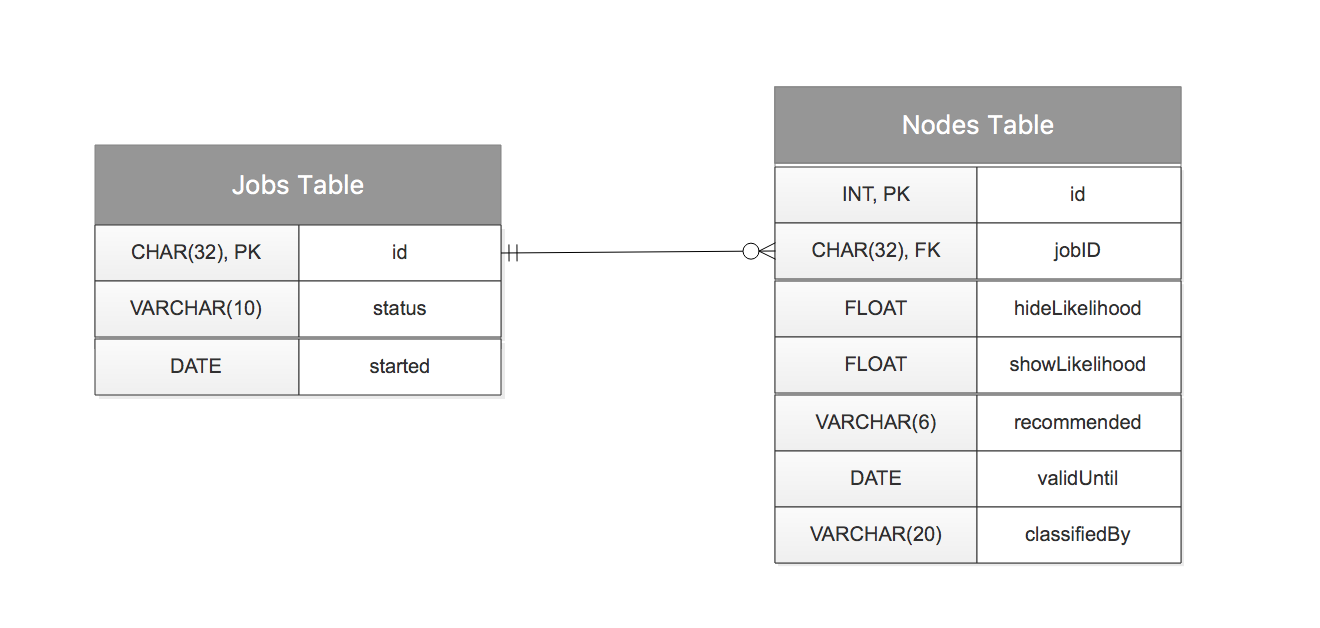
\includegraphics[width=.7\textwidth]{graphics/cache-schema}
		\caption[Cache schema]{Figure showing the relational schema used by the caching mechanism}
		\label{Fig: impl/REST/cache/relational}
	\end{figure}
	\section{}
\end{document}

%%%%%%%%%%%%%%%%%%%%%%%%%%%%%%%%%%%%
%%%%%%%%%%%%%  EVALUATION %%%%%%%%%%%%%
%%%%%%%%%%%%%%%%%%%%%%%%%%%%%%%%%%%%
\begin{document}
	\chapter{Evaluation}
	\section{Success criteria} \label{Section: eval/success-criteria}
		blah
	\section{Features evaluation} \label{Section: eval/features}
		Even though the key module of the entire project was the one where the machine learning models are implemented, the set of features extracted for each node is at least as important because, without them being representative, the models will not be able to generalize well. For this reason, in this section, I will present the evaluation of the features I extracted for each node.
		
	\subsection{Feature importance algorithm} \label{Section: eval/features/alg}
		In order to measure the feature importance I made use of the Boruta algorithm, proposed by \textit{M. Kursa et al.}\cite{JSSv036i11}. It uses a random forest classification in order to compute the \textbf{z score} for every feature taken into consideration. 
		\\ \\
		In short, the algorithm is based on the same idea which forms the foundation of a random forest classifier, namely, that by adding randomness to the system and collecting results from the ensemble of randomized samples one can reduce the misleading impact of random fluctuations and correlations. In this case, this extra randomness provides a clearer view of which features really are important. The steps enumerated below are repeated until either the importance is assigned for all features or the algorithm has reached the previously set limit of random forests runs:
		\begin{enumerate}
			\item Extend the feature space by adding copies of all variables and then shuffle the added attributes in order to remove their correlations with the response.
			\item Run a random forest classifier on the extended dataset and gather the z-scores computed.
			\item Find the maximum z-score among the shadow features (MZSA) and assign a hit to every feature that scored better than MZSA
			\item For each feature with undetermined importance perform a two-sided equality test with MZSA
			\item Consider the features with importance significantly lower than MZSA as \textit{unimportant} and the ones with importance significantly higher than MZSA as \textit{important}.
			\item Remove all shadow attributes
		\end{enumerate}
	\subsection{Results \& discussion} \label{Section: eval/features/results}
		
	\section{Evaluation of machine learning models} \label{Section: eval/ml}
	\subsection{Evaluation methodology} \label{Section: eval/ml/methodology}
		In order to quantitatively evaluate the performance of the machine learning models implemented, I used a labelled dataset $\mathbf{s}$ containing $5,498$ nodes. Figure \ref{Fig: eval/ml/methodology/dist} shows how the labels and node types are distributed in the dataset used in this case. From there, we can observe that the node type distribution resembles the distribution that can be found in the general case in a provenance graph. Therefore, by evaluating the models on this dataset I can produce a comprehensive and accurate assessment of their performance. 
		\begin{figure}[H]
			\centering
			\begin{subfigure}{.4\textwidth}
				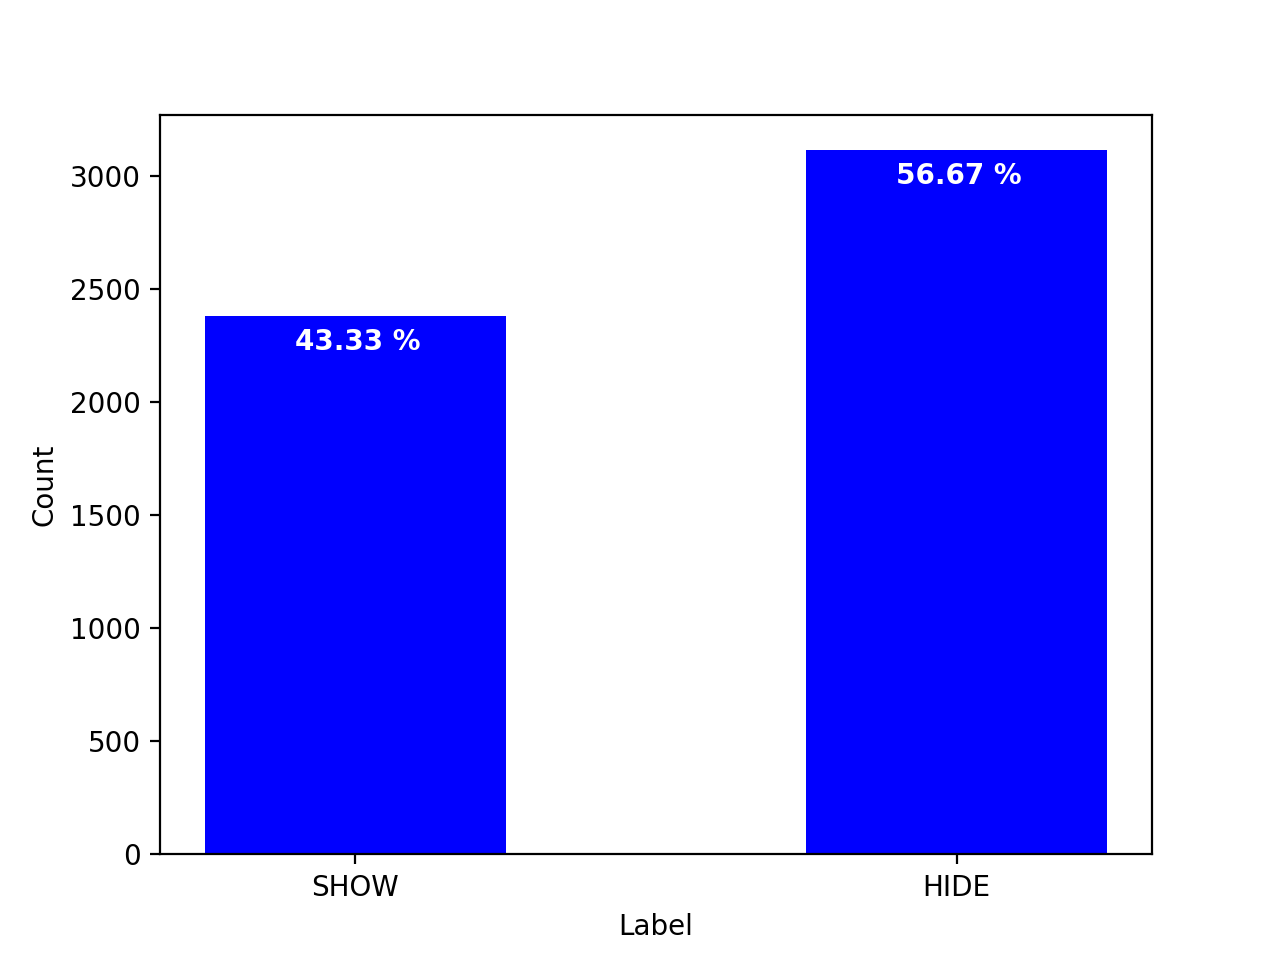
\includegraphics[width=\textwidth]{graphics/labels-dist}
			\end{subfigure}
			\hfill
			\begin{subfigure}{.4\textwidth}
				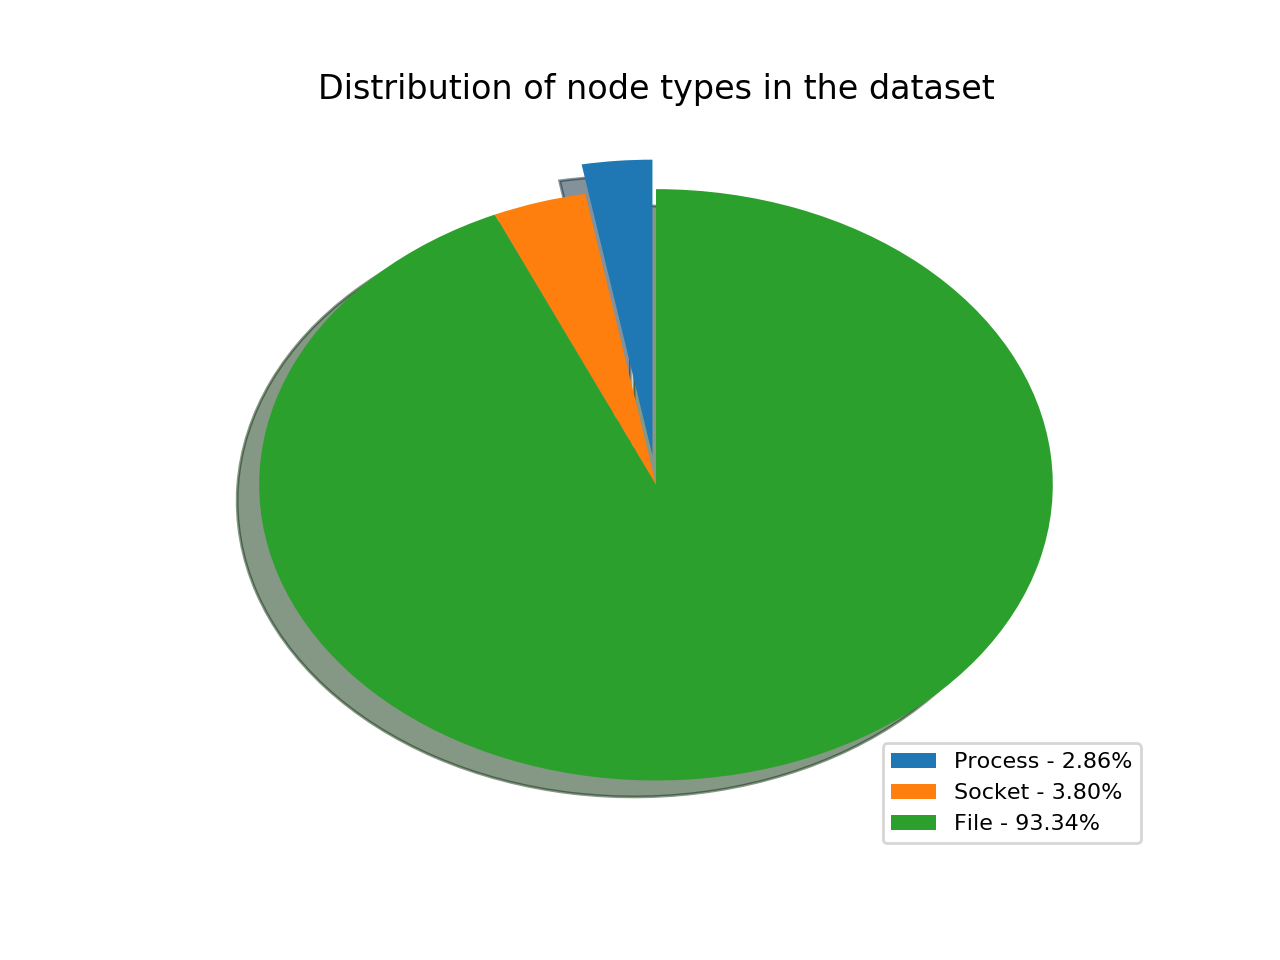
\includegraphics[width=\textwidth]{graphics/node-dist}
			\end{subfigure}
			\caption[Distributions of labels and node type in the dataset]{\textit{Left:} Distribution of the labels in the dataset. \textit{Right: }Distribution of the node types in the dataset.}
			\label{Fig: eval/ml/methodology/dist}
		\end{figure} 
		The technique used when evaluating the models was \textbf{k-fold cross validation}. Essentially, I split the dataset in $10$ equally-sized slots and use one at a time as a test set, while the other $9$ serve as the training set for the model. Figure \ref{Fig: impl/ml/methodology/kfold/first} shows how the dataset is divided in the first iteration of the cross-validation algorithm. For the models that require a validation set for optimising hyperparameters, the training set is split again in $10$ slots of equal sizes and uses one at a time as a validation set. This way, I ensure that none of the models is not tested on previously-seen examples and therefore I correctly evaluate how well they generalize on the given data.
		\begin{figure}[H]
			\centering
			\includegraphics[width=.8\textwidth]{graphics/k-fold}
			\caption{First step in k-fold cross validation}
			\label{Fig: impl/ml/methodology/kfold/first}
		\end{figure}
		
		At every iteration, I compute a set of metrics that for estimating the model's performance and the final result for every metric in part is given by averaging over the values obtained. 
	\subsection{Metrics involved} \label{Section: eval/ml/metrics}
	
		In this section, I will outline the metrics used when evaluating the machine learning models. The choice of good metrics is essential when comparatively evaluating a number of machine learning models. The simplest metric for evaluating of classification algorithms is \textbf{accuracy}, and can be computed using the formula: 
		\\
		\begin{equation}
			acc = \frac{\text{no. of correctly predicted nodes}}{\text{total no. of predicted nodes}}
		\end{equation}
		\\
		Accuracy, however, is not efficient when it comes to imbalanced data, as it is the case here(i.e. we have a $43\%/57\%$ \textit{SHOW/HIDE} distribution amongst the nodes). Therefore, more complex metrics are required in order to correctly assess the performance of the models implemented. These metrics are based on the notions of \textit{true positives, true negatives, false positives and false negatives}, which can easily be illustrated using a confusion matrix, such as the one from Figure \ref{Fig: eval/ml/metrics/confusion-matrix}.
		\begin{figure}[H]
			\centering
			\includegraphics[width=.7\textwidth]{graphics/confusion-matrix}
			\caption{Confusion matrix for two-class classification}
			\label{Fig: eval/ml/metrics/confusion-matrix}
		\end{figure}
		The metrics I used to evaluate the general performance of the models are presented in Table \ref{Table: eval/ml/metrics/metrics}. From those, the F1 score and the MCC are the most meaningful for this case, as they ignore the fact that the data is not balanced. The F1 score gives a value in the interval $[0, 1]$, with $1$ representing perfect prediction, while the MCC gives a value between $[-1, 1]$, where $1$ represents perfect prediction, $0$ not better than random and $-1$ a total disagreement between the predicted and true labels.
		\begin{longtable}{|p{.15\textwidth}|p{.40\textwidth}|c|}
		   \textbf{Metric} & \textbf{Intuition} &\textbf{Formula} \\
			\hline
			\textit{Precision} & fraction of nodes correctly labelled as \textit{SHOW} in all nodes classified. & {$\centering \text{precision} = \frac{tp}{tp+fp}$} \\
			\hline 
			\textit{Recall} & fraction of \textit{SHOW} nodes correctly classified. & $\text{recall} = \frac{tp}{tp+fn}$ \\
			\hline
			\textit{F1 score} & takes into consideration both the precision and the recall of the model in order to assess its performance & $\text{F1} = 2\times\frac{\text{precision}\times\text{recall}}{\text{precision} + \text{recall}}$\\
			\hline 
			\textit{Matthew's Correlation Coefficient (MCC)} & takes into account true and false positives and negatives in order to provide a balanced metric for the model's performance & $MCC = \frac{tp\times tn - fp\times fn}{\sqrt{(tp+fp)\times(tp+fn)\times(tn+fp)\times(tn+fn)}}$\\
			\hline
			\caption{Machine learning evaluation metrics}
			\label{Table: eval/ml/metrics/metrics}
		\end{longtable}
		
		\subsection{Results \& discussion} \label{Section: eval/ml/results}

		\section{Service time evaluation} \label{Section: eval/service-time}
			This project is meant to be a complete API that can be used in practice by the CADETS user interface. Therefore, besides the performance of the machine learning model used, it is essential to evaluate it in terms of the service speed as well. All the timing results were obtained using my personal machine. For a job processing $N$ nodes, the service time is calculated using the following formula:  
			\begin{equation}
				\text{service\_time} = N\times [CCT + CHR \times CET + (1-CHR) \times (CT + RCT)] + MLT
				\label{Eq: eval/service-time/overall}
			\end{equation}
			where: 
			\begin{itemize}
				\item $\mathbf{CCT} \in \mathbb{R}$ = Cache Check Time - time taking to check if a node is in the cache database and if the entry is still valid.
				\item $\mathbf{CHR} \in [0, 1]$ = Cache Hit Rate.
				\item $\textbf{CET} \in \mathbb{R}$ = Cache Extraction Time - time taking to extracted one cached result.
				\item $\textbf{CT} \in \mathbb{R}$ = Classification Time - time taking to classify a node. 
				\item $\textbf{RCT} \in \mathbb{R}$ = Result Caching Time - time required to add a new classification result to the cache database.
				\item $\mathbf{MLT} \in \mathbb{R}$ = Model Loading Time - time required to configure the model (i.e. defining its components and load the corresponding pre-optimised parameters)
			\end{itemize}
			In practice, the API is expected to re-use many of the classification results. For this reason, I assume the the cache to have a hit-rate $CHR = 90\%$. For simulation purposes, the database was populated with $10, 000$ nodes and $30$ completed jobs, each having processed $1, 000$ nodes. 
			\\ \\
			The first step performed by the application when the new job is initiated is to check the cache and try to get the nodes that are cached. In this given simulation environment, the Cache Check Time, Cache Extraction Time and Result Caching Time are $CCT=??????????$, $CET=???????????$ and $RCT=??????????????$, respectively.  
			
		\subsection{Classification timings} \label{Section: eval/service-time/classification}
			The classification time is not as straight-forward as the times shown so far. It was computed using the following formula:
			\begin{equation}
				CT = NTT + FET + MRT
			\end{equation}
			where: 
			\begin{itemize}
				\item $\mathbf{NTT} \in \mathbb{R}$ = Node Type Time - time required to get the node type
				\item $\mathbf{FET} \in \mathbb{R}$ = Feature Extraction Time - time required to extract the features required for a node.
				\item $\mathbf{MRT} \in \mathbb{R}$ = Model Running Time - time required for the model to produce a classification result for a node.
			\end{itemize}
			If a node is not in the cache, we first need to get the node type. The feature extraction time is dependent on this, as different node types require a slightly different feature extraction algorithm. Moreover, for a \textit{Meta} or \textit{Pipe} node, we also need to look for the closest \textit{Process} node to them. Table \ref{Table: eval/service-time/classification/fet} shows a breakdown of these timings, when the nodes are extracted from a database of $6,008$ nodes and taking into account the policy defined in Section \ref{Section: impl/REST/actual} from the Implementation chapter.
			\begin{longtable}{|p{.1\textwidth} || p{.15\textwidth} | p{.20\textwidth}| p{.15\textwidth}| p{.20\textwidth} | }
				\textbf{Node type} & \textbf{NTT} (s) & \textbf{Extra time} (s)& \textbf{FET} (s)& \textbf{Total FET} (s)\\
				\hline
				\textit{File} & & $0.0$ & & \\
				\textit{Process} & & $0.0$ & & \\
				\textit{Socket} & & $0.0$ & & \\
				\textit{Meta} & & & & \\
				\textit{Pipe} & & & & \\
				\textit{Machine} & & $0.0$ & $0.0$ & \\
				\hline
				\caption{Breakdown of feature extraction times}
				\label{Table: eval/service-time/classification/fet}
			\end{longtable}
			
			Once the feature vectors are computed, they are passed to the machine learning models to be classified. Based on the model type, this task can take different amounts of time. Table \ref{Table: eval/service-time/classification/MRT} shows a breakdown of Model Load Time(MLT) and Model Running Time(MRT), based on the model type. 
			
			\begin{longtable}{|p{.15\textwidth}||p{.15\textwidth}|p{.15\textwidth}|p{.15\textwidth}|p{.15\textwidth}|p{.15\textwidth}|}
				\textbf{Model} & \textit{Logistic Regression} & \textit{MLP} & \textit{CNN} & \textit{GAT} & \textit{PNN} \\
				\hline
				\textbf{MLT} (s) & & & & & \\
				\hline
				\textbf{MRT} (s) & & & & & \\
				\hline
				\caption{Breakdown of model running times}
				\label{Table: eval/service-time/classification/MRT}
			\end{longtable} 
			The classification time can then be written as a function of node and model type as follows:
			\begin{equation}
				CT(nt, mt) = Total\_FET(nt) + MRT(mt)
			\end{equation}
			By using the node type distribution outlined in the histogram from Figure \ref{Figure 2.1.1}, I can compute the average classification time as a function of model type:
			\begin{equation}
				\hat{CT}(mt) = \sum_{nt\in \mathbf{\mathcal{N}}} (\mathbb{P}(nt) \times Total\_FET(nt)) + MRT(mt) 
			\end{equation}  
			where $\mathcal{N}$ is the set of available node types. Table \ref{Table: eval/service-time/classification/CT} shows the results of the average classification times for each model. 
			
			\begin{longtable}{|p{.15\textwidth}||p{.15\textwidth}|p{.15\textwidth}|p{.15\textwidth}|p{.15\textwidth}|p{.15\textwidth}|}
				\textbf{Model} & \textit{Logistic Regression} & \textit{MLP} & \textit{CNN} & \textit{GAT} & \textit{PNN} \\
				\hline
				$\mathbf{\hat{CT}}$ (s) & & & & & \\
				\hline
				\caption{Breakdown of average classification times.}
				\label{Table: eval/service-time/classification/CT}
			\end{longtable}
			
			\subsection{Bringing it all together} \label{Section: eval/service-time/together}
			Now that I have computed all the individual time values, I can bring them all together and compute the \textit{service time}, using Eq. \ref{Eq: eval/service-time/overall}. Table \ref{Table: eval/service-time/together/overall} shows the resulting service times for different model types, taking the number of nodes $N=1,000$.
			\begin{longtable}{|p{.13\textwidth}||p{.1\textwidth}|p{.1\textwidth}|p{.1\textwidth}|p{.1\textwidth}|p{.1\textwidth}|p{.1\textwidth}||p{.1\textwidth}|}
				\textbf{Model} & \textbf{N} & \textbf{CHR} & \textbf{CCT} (s)  & \textbf{RCT} (s)& $\mathbf{\hat{CT}}$ (s)& \textbf{MLT} (s)& \textbf{Total} (s)\\
				\hline
				\textit{Logistic Regression} & \multirow{5}{*}{$1000$} & \multirow{5}{*}{$0.90$} & \multirow{5}{*}{$0.0$} & \multirow{5}{*}{$0.0$} & $0.0$ & $0.0$ & \cellcolor{green!20} $\mathbf{0.0}$ \\
				\hhline{-~~~~---}
				\textit{MLP} &  &  &  &  & $0.0$ & $0.0$ &\cellcolor{green!20} $\mathbf{0.0}$  \\
				\hhline{-~~~~---}
				\textit{CNN} &  &  &  &  & $0.0$ & $0.0$ & \cellcolor{green!20} $\mathbf{0.0}$ \\
				\hhline{-~~~~---}
				\textit{GAT} &  &  &  & & $0.0$ & $0.0$ & \cellcolor{green!20} $\mathbf{0.0}$ \\
				\hhline{-~~~~---}
				\textit{PNN} &  &  &  &  & $0.0$ & $0.0$ & \cellcolor{green!20} $\mathbf{0.0}$ \\
				\hline
				\caption{Service time analysis results}
				\label{Table: eval/service-time/together/overall}
			\end{longtable}
			{\LARGE \textbf{INCLUDE DISCUSSION}}
		\section{Summary} \label{Section: eval/summary}
\end{document}

%%%%%%%%%%%%%%%%%%%%%%%%%%%%%%%%%%%%
%%%%%%%%%%%%%  CONCLUSION %%%%%%%%%%%%%
%%%%%%%%%%%%%%%%%%%%%%%%%%%%%%%%%%%%
\begin{document}
	\chapter{Conclusion}
		In this dissertation, I have outlined the work done in designing, implementing and evaluating a machine-learning based extension for the CADETS UI with the purpose of filtering graph-structured OS-level provenance data. It classifies the nodes either into nodes that are of interest or nodes that are not of interest, from a cybersecurity perspective. As expected, by analysing several datasets, I observed that these two classes are highly imbalanced (i.e. there are more nodes that don't represent a potential threat than nodes that do). This imbalance in the data labels and the fact that there are multiple node types that had to be represented added a degree of complexity to the problem at hand. Through this dissertation, I have shown how these difficulties were overcome using suitable pre-processing techniques and machine learning models. 
		\\ \\
		The project requirements were all successfully achieved and a set of extensions were implemented. The evaluation of the models analyses both their performance (using a number of standard metrics) and their applicability to the problem at hand. 
		
	\section{Lessons learnt} 
		This project gave me the opportunity to explore several machine learning techniques, both parametric and non-parametric, and how they can be applied to real-world data. The Neo4J-stored graph cannot be passed directly to the machine learning models. For this reason, I also explored a few data processing techniques in order to come up with a feature vector representation for every node. Finally, I explored different API architectures that would allow the machine learning models to run as an independent entity, for the CADETS UI to make requests to.
		\\ \\
		Because the machine learning models represent the core module of this project and each model in part underwent continuous fine-tuning, the iterative and incremental development model has proven to be appropriate choice for the project at hand. Using Python as the main programming language was also appropriate, having support for data processing and machine learning development through libraries such as Numpy and Keras. Moreover, it also provides support for handling incoming network requests through the Flask library, essential in developing the REST API that wraps around the machine learning models.
		\\ \\
		If I were to do the project again, I would allow even more time to exploring different machine learning techniques, so that I could implement models that use even more of the relational nature of the graph data. On top of that, I would have allowed more time to fine-tuning the neural networks, given the fact that a performant machine learning model does not require a predefined set of steps, but it is rather a matter of trial and error.
	\section{Further work}
		Working on this project gave me the opportunity to explore areas of Computer Science that were intriguing, but still very little known to me. Personally, I find that this was an extraordinary learning experience and I consider the project a success. However, there are many possible extensions that can be implemented in order to make it even more successful, including:
		\begin{enumerate}
			\item \textit{Exploring more complex neural networks} - Machine learning applied on graphs is a current research trend, with more and more architectures being designed specifically for graph-structured data. Implementing one of these NN architectures would allow me to make more use of the relational nature of the data than I currently do. Two of the models that I would like to implement are Graph Convolutional Networks \cite{kipf2017semi} and Graph Attention Networks \cite{2017arXiv171010903V}.
			
			\item \textit{Solving the Neo4J access bottleneck} - Overcome the low time performance of the library that facilitates the Neo4J connection. One potential solution would be to replicate the database over multiple instances and perform the feature extraction in parallel. 
				
			\item \textit{Implementing machine learning models that can adapt to user input} - In the final stage, the machine learning models filtering the graph data should accept and adapt from user input, rather than just using a set of predefined rules. The logical next step would be to extend the models such as they can support this, while preserving their performance.
	\end{enumerate}
	
\end{document}

%%%%%%%%%%%%%%%%%%%%%%%%%%%%%%%%%%%%
%%%%%%%%%%%%%  APPENDIX A %%%%%%%%%%%%%
%%%%%%%%%%%%%%%%%%%%%%%%%%%%%%%%%%%%
\appendix

%%%%%%%%%%%%%%%%%%%%%%%%%%%%%%%%%%%%
%%%%%%%%%%%%%  BIBLIOGRAPHY %%%%%%%%%%%%%
%%%%%%%%%%%%%%%%%%%%%%%%%%%%%%%%%%%%
\addcontentsline{toc}{chapter}{Bibliography}
\bibliography{refs}
\nocite{pnn, polonium, pnn-parallel, sigmoidal, nonlinearities, DBLP:journals/corr/LuongPM15, 7266837, 2017arXiv171010903V, 279181, DBLP:journals/corr/KingmaB14, DBLP:journals/corr/VaswaniSPUJGKP17, REST-general, chollet2015keras, DBLP:journals/corr/IoffeS15, Rutkowski2004}
\chapter{Neural Network optimization} \label{appendix-MLP-opt}
In this appendix, I will outline two algorithms that can be used for optimising a neural network.
\section{Gradient descent}
In this section, I will describe the inner-workings of the most popular optimization algorithm for machine learning models, \textbf{gradient descent}. It is an iterative algorithm that finds the optimal weights and biases by minimizing a given loss function $\mathfrak{L}(\mathbf{x}_i, \mathbf{y}_i, \mathbf{w}, \mathbf{b})$.
\\ \\
Let $\mathbf{s}$ be a set of training examples $\mathbf{s}=(\mathbf{X}, \mathbf{Y})$, where $\mathbf{X} = [\mathbf{x_1}\dots\mathbf{x_m}]$ is the matrix of training feature vectors, with $\mathbf{x_i}\in\mathbb{R}^n. \forall i \in \{1\dots m\}$ and $\mathbf{Y} = [\mathbf{y_1}\dots\mathbf{y_m}]$ is the matrix representing the corresponding class for every input feature vector, using one-hot encoding. For an input vector $\mathbf{x_i}$ in class $C_t$, the corresponding $\mathbf{y_i}$ will be:
\begin{equation}
\centering
\mathbf{y_i}^T = [y_{i, 1}\dots y_{i, k}]
\end{equation} 
where:
\begin{equation}
\centering
y_{i, j} = 
\begin{cases}
1 & \text{if } j = t \\
0 & \text{otherwise}
\end{cases}
\end{equation}
The choice of the loss function depends on the network infrastructure and the problem it is trying to solve. One of the most popular loss functions for classification problems is \textbf{cross-entropy}. It computes the difference between the true output distribution $\mathbf{y}_i$ and the neural network output distribution $\mathbf{\hat{y}}_i$, respectively:
\begin{equation}
\centering
\mathfrak{L}(\mathbf{x}_i, \mathbf{y}_i, \mathbf{w}, \mathbf{b}) = -\sum_{j=1}^{k}y_{i,j}\log(\hat{y}_{i,j})
\end{equation}
In order to avoid potential overfitting of the model to the training data, one may change the loss function such that it includes the norm of the weights vector:
\begin{equation}
\mathfrak{L}(\mathbf{x}_i, \mathbf{y}_i, \mathbf{w}, \mathbf{b}) = -\sum_{j=1}^{k}y_{i,j}\log(\hat{y}_{i,j}) + \vert\vert \mathbf{w} \vert\vert
\end{equation} 
The gradient descent algorithm then updates the weights and biases as follows: 
\begin{equation}
\centering
\mathbf{w}_{t+1} \leftarrow \mathbf{w}_t - \alpha \sum_{i=1}^{m}\frac{\partial \mathfrak{L}}{\partial \mathbf{w}}\Bigr|_{\substack{\mathbf{w}_t}}
\label{Eq: gdes/update/weights}
\end{equation}
\begin{equation}
\centering
\mathbf{b}_{t+1} \leftarrow \mathbf{b}_t - \alpha \sum_{i=1}^{m}\frac{\partial \mathfrak{L}}{\partial \mathbf{b}}\Bigr|_{\substack{\mathbf{b}_t}}
\label{Eq: gdes/update/weigts}
\end{equation}
where $\mathbf{w}_t$ and $\mathbf{b}_t$ are the weights and biases at iteration t, $\mathfrak{L} = \mathfrak{L}(\mathbf{x}_i, \mathbf{y}_i, \mathbf{w}_t, \mathbf{b}_t)$ and $\alpha$ is the learning rate - a hyperparameter that decides the amount by which the direction of the gradient is followed at each iteration. The value of the learning rate impacts the behaviour of the optimisation algorithm. A high learning rate might cause the algorithm to never reach the minimum of the loss function. The lower it is, the slower we travel along the downwards slope of the loss function. Even though this ensures the fact that we don't miss any local minima, it can also mean that the algorithm will take a long time to converge - especially if it gets stuck on a plateau region. 
\\ \\
\textbf{Backpropagation} is the technique used to compute the gradient of the loss function with respect with the weights $\mathbf{w}$ and biases $\mathbf{b}$. The overall algorithm has two phases:
\begin{itemize}
	\item Phase 1: \textbf{Propagation}
	\begin{enumerate}
		\item Propagate every training example $\mathbf{x}_i$ through the network to generate the output values $\mathbf{\hat{y}}_i$.
		\item Calculate the loss function $\mathfrak{L}$.
		\item Backpropagate the output activations back through the network using the training pattern in order to generate the gradients of all output and hidden neurons.
	\end{enumerate}
	\item Phase 2: \textbf{Weights and biases updating}, using the equations \ref{Eq 2.13} and \ref{Eq 2.14}
\end{itemize}
\textbf{Mini-batch gradient descent} is a variation of gradient descent that splits the training set into small batches $\mathfrak{B}=\{(\mathbf{x}_1, \mathbf{y}_1)\dots(\mathbf{x}_l, \mathbf{y}_l)\}$. Each batch $\mathfrak{B}$ is used to calculate the loss function and update model coefficients. The coefficients update frequency is higher than classical gradient descent which allows for a more robust convergence, avoiding local minima. 

\section{Adam} \label{Appendix: Adam}

Given the gradient of the loss function with respect to the weights over a mini-batch $\mathfrak{B}$ at timestep t: 

\begin{equation}
\mathbf{g}_t = 
\sum_{(\mathbf{x}, \mathbf{y} \in \mathfrak{B})}
\frac{
	\partial \mathfrak(\mathbf{w}, \mathbf{b}, \mathbf{x}, \mathbf{y})
}{
	\partial \mathbf{w}
},
\end{equation}
it computes an exponentially decaying average of previous gradients $\mathbf{m}_t$ and an exponentially decaying average of previous squared gradients $\mathbf{v}_t$:
\begin{equation}
\mathbf{m}_t = \beta_1 \mathbf{m}_{t-1} + (1-\beta_1)\mathbf{g}_t 
\end{equation}
\begin{equation}
\mathbf{v}_t = \beta_2 \mathbf{v}_{t-1} + (1-\beta_2)\mathbf{g}_t^2 
\end{equation}
where $\beta_1$ and $\beta_2$ are the exponential decaying rates, usually set to $\beta_1 = 0.9$ and $\beta_2 = 0.999$. As $\mathbf{m}_t$ and $\mathbf{v}_t$ are initialised to $0$, the optimiser applies the following corrections: 
\begin{equation}
\mathbf{\hat{m}}_t = \frac{\mathbf{m}_t}{1-\beta_1^t}
\end{equation}
\begin{equation}
\mathbf{\hat{v}}_t = \frac{\mathbf{v}_t}{1-\beta_2^t}
\end{equation}

\chapter{Adam} \label{Appendix: Adam}

Given the gradient of the loss function with respect to the weights over a mini-batch $\mathfrak{B}$ at timestep t: 

\begin{equation}
\mathbf{g}_t = 
\sum_{(\mathbf{x}, \mathbf{y} \in \mathfrak{B})}
\frac{
	\partial \mathfrak(\mathbf{w}, \mathbf{b}, \mathbf{x}, \mathbf{y})
}{
	\partial \mathbf{w}
},
\end{equation}
it computes an exponentially decaying average of previous gradients $\mathbf{m}_t$ and an exponentially decaying average of previous squared gradients $\mathbf{v}_t$:
\begin{equation}
\mathbf{m}_t = \beta_1 \mathbf{m}_{t-1} + (1-\beta_1)\mathbf{g}_t 
\end{equation}
\begin{equation}
\mathbf{v}_t = \beta_2 \mathbf{v}_{t-1} + (1-\beta_2)\mathbf{g}_t^2 
\end{equation}
where $\beta_1$ and $\beta_2$ are the exponential decaying rates, usually set to $\beta_1 = 0.9$ and $\beta_2 = 0.999$. As $\mathbf{m}_t$ and $\mathbf{v}_t$ are initialised to $0$, the optimiser applies the following corrections: 
\begin{equation}
\mathbf{\hat{m}}_t = \frac{\mathbf{m}_t}{1-\beta_1^t}
\end{equation}
\begin{equation}
\mathbf{\hat{v}}_t = \frac{\mathbf{v}_t}{1-\beta_2^t}
\end{equation}

\end{document}